\documentclass[a4paper]{article}

\def\npart {III}
\def\nterm {Lent}
\def\nyear {2017}
\def\nlecturer {B.\ P.\ Narayanan}
\def\ncourse {Ramsey Theory}

% Imports
\ifx \nextra \undefined
  \usepackage[pdftex,
    hidelinks,
    pdfauthor={Dexter Chua},
    pdfsubject={Cambridge Maths Notes: Part \npart\ - \ncourse},
    pdftitle={Part \npart\ - \ncourse},
  pdfkeywords={Cambridge Mathematics Maths Math \npart\ \nterm\ \nyear\ \ncourse}]{hyperref}
  \title{Part \npart\ - \ncourse}
\else
  \usepackage[pdftex,
    hidelinks,
    pdfauthor={Dexter Chua},
    pdfsubject={Cambridge Maths Notes: Part \npart\ - \ncourse\ (\nextra)},
    pdftitle={Part \npart\ - \ncourse\ (\nextra)},
  pdfkeywords={Cambridge Mathematics Maths Math \npart\ \nterm\ \nyear\ \ncourse\ \nextra}]{hyperref}

  \title{Part \npart\ - \ncourse \\ {\Large \nextra}}
\fi

\author{Lectured by \nlecturer \\\small Notes taken by Dexter Chua}
\date{\nterm\ \nyear}

\usepackage{alltt}
\usepackage{amsfonts}
\usepackage{amsmath}
\usepackage{amssymb}
\usepackage{amsthm}
\usepackage{booktabs}
\usepackage{caption}
\usepackage{enumitem}
\usepackage{fancyhdr}
\usepackage{graphicx}
\usepackage{mathtools}
\usepackage{microtype}
\usepackage{multirow}
\usepackage{pdflscape}
\usepackage{pgfplots}
\usepackage{siunitx}
\usepackage{tabularx}
\usepackage{tikz}
\usepackage{tkz-euclide}
\usepackage[normalem]{ulem}
\usepackage[all]{xy}

\pgfplotsset{compat=1.12}

\pagestyle{fancyplain}
\lhead{\emph{\nouppercase{\leftmark}}}
\ifx \nextra \undefined
  \rhead{
    \ifnum\thepage=1
    \else
      \npart\ \ncourse
    \fi}
\else
  \rhead{
    \ifnum\thepage=1
    \else
      \npart\ \ncourse\ (\nextra)
    \fi}
\fi
\usetikzlibrary{arrows}
\usetikzlibrary{decorations.markings}
\usetikzlibrary{decorations.pathmorphing}
\usetikzlibrary{positioning}
\usetikzlibrary{fadings}
\usetikzlibrary{intersections}
\usetikzlibrary{cd}

\newcommand*{\Cdot}{\raisebox{-0.25ex}{\scalebox{1.5}{$\cdot$}}}
\newcommand {\pd}[2][ ]{
  \ifx #1 { }
    \frac{\partial}{\partial #2}
  \else
    \frac{\partial^{#1}}{\partial #2^{#1}}
  \fi
}

% Theorems
\theoremstyle{definition}
\newtheorem*{aim}{Aim}
\newtheorem*{axiom}{Axiom}
\newtheorem*{claim}{Claim}
\newtheorem*{cor}{Corollary}
\newtheorem*{defi}{Definition}
\newtheorem*{eg}{Example}
\newtheorem*{fact}{Fact}
\newtheorem*{law}{Law}
\newtheorem*{lemma}{Lemma}
\newtheorem*{notation}{Notation}
\newtheorem*{prop}{Proposition}
\newtheorem*{thm}{Theorem}

\renewcommand{\labelitemi}{--}
\renewcommand{\labelitemii}{$\circ$}
\renewcommand{\labelenumi}{(\roman{*})}

\let\stdsection\section
\renewcommand\section{\newpage\stdsection}

% Strike through
\def\st{\bgroup \ULdepth=-.55ex \ULset}

% Maths symbols
\newcommand{\bra}{\langle}
\newcommand{\ket}{\rangle}

\newcommand{\N}{\mathbb{N}}
\newcommand{\Z}{\mathbb{Z}}
\newcommand{\Q}{\mathbb{Q}}
\renewcommand{\H}{\mathbb{H}}
\newcommand{\R}{\mathbb{R}}
\newcommand{\C}{\mathbb{C}}
\newcommand{\Prob}{\mathbb{P}}
\renewcommand{\P}{\mathbb{P}}
\newcommand{\E}{\mathbb{E}}
\newcommand{\F}{\mathbb{F}}
\newcommand{\cU}{\mathcal{U}}
\newcommand{\RP}{\mathbb{RP}}
\newcommand{\CP}{\mathbb{CP}}

\newcommand{\ph}{\,\cdot\,}

\DeclareMathOperator{\sech}{sech}
\DeclareMathOperator{\cosech}{cosech}
\DeclareMathOperator{\cosec}{cosec}

\DeclareMathOperator{\covol}{covol}
\DeclareMathOperator{\vol}{vol}

\let\Im\relax
\let\Re\relax
\DeclareMathOperator{\Im}{Im}
\DeclareMathOperator{\Re}{Re}
\DeclareMathOperator{\im}{im}
\DeclareMathOperator{\image}{image}
\DeclareMathOperator{\Ann}{Ann}

\DeclareMathOperator*{\res}{res}
\DeclareMathOperator{\Res}{Res}
\DeclareMathOperator{\Ind}{Ind}

\DeclareMathOperator{\tr}{tr}
\DeclareMathOperator{\diag}{diag}
\DeclareMathOperator{\rank}{rank}
\DeclareMathOperator{\card}{card}
\DeclareMathOperator{\spn}{span}
\DeclareMathOperator{\adj}{adj}

\DeclareMathOperator{\erf}{erf}
\DeclareMathOperator{\erfc}{erfc}

\DeclareMathOperator{\ord}{ord}
\DeclareMathOperator{\Sym}{Sym}

\DeclareMathOperator{\sgn}{sgn}
\DeclareMathOperator{\orb}{orb}
\DeclareMathOperator{\stab}{stab}
\DeclareMathOperator{\ccl}{ccl}

\DeclareMathOperator{\lcm}{lcm}
\DeclareMathOperator{\hcf}{hcf}

\DeclareMathOperator{\Int}{Int}
\DeclareMathOperator{\id}{id}

\DeclareMathOperator{\betaD}{beta}
\DeclareMathOperator{\gammaD}{gamma}
\DeclareMathOperator{\Poisson}{Poisson}
\DeclareMathOperator{\binomial}{binomial}
\DeclareMathOperator{\multinomial}{multinomial}
\DeclareMathOperator{\Bernoulli}{Bernoulli}
\DeclareMathOperator{\like}{like}

\DeclareMathOperator{\var}{var}
\DeclareMathOperator{\cov}{cov}
\DeclareMathOperator{\bias}{bias}
\DeclareMathOperator{\mse}{mse}
\DeclareMathOperator{\corr}{corr}

\DeclareMathOperator{\otp}{otp}
\DeclareMathOperator{\dom}{dom}

\DeclareMathOperator{\Root}{Root}
\DeclareMathOperator{\supp}{supp}
\DeclareMathOperator{\rel}{rel}
\DeclareMathOperator{\Hom}{Hom}
\DeclareMathOperator{\Aut}{Aut}
\DeclareMathOperator{\Gal}{Gal}
\DeclareMathOperator{\Mat}{Mat}
\DeclareMathOperator{\End}{End}
\DeclareMathOperator{\Char}{char}
\DeclareMathOperator{\ev}{ev}
\DeclareMathOperator{\St}{St}
\DeclareMathOperator{\Lk}{Lk}
\DeclareMathOperator{\disc}{disc}
\DeclareMathOperator{\Isom}{Isom}
\DeclareMathOperator{\length}{length}
\DeclareMathOperator{\energy}{energy}
\DeclareMathOperator{\area}{area}
\DeclareMathOperator{\Syl}{Syl}
\DeclareMathOperator{\cl}{cl}
\DeclareMathOperator{\fix}{fix}

\newcommand{\GL}{\mathrm{GL}}
\newcommand{\SL}{\mathrm{SL}}
\newcommand{\PGL}{\mathrm{PGL}}
\newcommand{\PSL}{\mathrm{PSL}}
\newcommand{\PSU}{\mathrm{PSU}}
\newcommand{\Or}{\mathrm{O}}
\newcommand{\SO}{\mathrm{SO}}
\newcommand{\U}{\mathrm{U}}
\newcommand{\SU}{\mathrm{SU}}

\renewcommand{\d}{\mathrm{d}}
\newcommand{\D}{\mathrm{D}}

\tikzset{->/.style = {decoration={markings,
                                  mark=at position 1 with {\arrow[scale=2]{latex'}}},
                      postaction={decorate}}}
\tikzset{<-/.style = {decoration={markings,
                                  mark=at position 0 with {\arrowreversed[scale=2]{latex'}}},
                      postaction={decorate}}}
\tikzset{<->/.style = {decoration={markings,
                                   mark=at position 0 with {\arrowreversed[scale=2]{latex'}},
                                   mark=at position 1 with {\arrow[scale=2]{latex'}}},
                       postaction={decorate}}}
\tikzset{->-/.style = {decoration={markings,
                                   mark=at position #1 with {\arrow[scale=2]{latex'}}},
                       postaction={decorate}}}
\tikzset{-<-/.style = {decoration={markings,
                                   mark=at position #1 with {\arrowreversed[scale=2]{latex'}}},
                       postaction={decorate}}}

\tikzset{circ/.style = {fill, circle, inner sep = 0, minimum size = 3}}
\tikzset{mstate/.style={circle, draw, blue, text=black, minimum width=0.7cm}}

\definecolor{mblue}{rgb}{0.2, 0.3, 0.8}
\definecolor{morange}{rgb}{1, 0.5, 0}
\definecolor{mgreen}{rgb}{0.1, 0.4, 0.2}
\definecolor{mred}{rgb}{0.5, 0, 0}

\def\drawcirculararc(#1,#2)(#3,#4)(#5,#6){%
    \pgfmathsetmacro\cA{(#1*#1+#2*#2-#3*#3-#4*#4)/2}%
    \pgfmathsetmacro\cB{(#1*#1+#2*#2-#5*#5-#6*#6)/2}%
    \pgfmathsetmacro\cy{(\cB*(#1-#3)-\cA*(#1-#5))/%
                        ((#2-#6)*(#1-#3)-(#2-#4)*(#1-#5))}%
    \pgfmathsetmacro\cx{(\cA-\cy*(#2-#4))/(#1-#3)}%
    \pgfmathsetmacro\cr{sqrt((#1-\cx)*(#1-\cx)+(#2-\cy)*(#2-\cy))}%
    \pgfmathsetmacro\cA{atan2(#2-\cy,#1-\cx)}%
    \pgfmathsetmacro\cB{atan2(#6-\cy,#5-\cx)}%
    \pgfmathparse{\cB<\cA}%
    \ifnum\pgfmathresult=1
        \pgfmathsetmacro\cB{\cB+360}%
    \fi
    \draw (#1,#2) arc (\cA:\cB:\cr);%
}
\newcommand\getCoord[3]{\newdimen{#1}\newdimen{#2}\pgfextractx{#1}{\pgfpointanchor{#3}{center}}\pgfextracty{#2}{\pgfpointanchor{#3}{center}}}

\def\Xint#1{\mathchoice
   {\XXint\displaystyle\textstyle{#1}}%
   {\XXint\textstyle\scriptstyle{#1}}%
   {\XXint\scriptstyle\scriptscriptstyle{#1}}%
   {\XXint\scriptscriptstyle\scriptscriptstyle{#1}}%
   \!\int}
\def\XXint#1#2#3{{\setbox0=\hbox{$#1{#2#3}{\int}$}
     \vcenter{\hbox{$#2#3$}}\kern-.5\wd0}}
\def\ddashint{\Xint=}
\def\dashint{\Xint-}


\DeclareMathOperator\Seq{Seq}
\begin{document}
\maketitle
{\small
\setlength{\parindent}{0em}
\setlength{\parskip}{1em}

What happens when we cut up a mathematical structure into many `pieces' ? How big must the original structure be in order to guarantee that at least one of the pieces has a specific property of interest? These are the kinds of questions at the heart of Ramsey theory. A prototypical result in the area is van der Waerden's theorem, which states that whenever we partition the natural numbers into finitely many classes, there is a class that contains arbitrarily long arithmetic progressions.

The course will cover both classical material and more recent developments in the subject. Some of the classical results that I shall cover include Ramsey's theorem, van der Waerden's theorem and the Hales--Jewett theorem; I shall discuss some applications of these results as well. More recent developments that I hope to cover include the properties of non-Ramsey graphs, topics in geometric Ramsey theory, and finally, connections between Ramsey theory and topological dynamics. I will also indicate a number of open problems.

\subsubsection*{Pre-requisites}
There are almost no pre-requisites and the material presented in this course will, by and large, be self-contained. However, students familiar with the basic notions of graph theory and point-set topology are bound to find the course easier.%
}
\tableofcontents

\setcounter{section}{-1}
\section{Introduction}
Vaguely, the main idea of Ramsey theory is as follows --- we have some object $X$ that comes with some structure, and then we break $X$ up into finitely many pieces. Can we find a piece that retains some of the structure of $X$? Usually, we phrase this in terms of \emph{colourings}. We pick a list of finitely many colours, and colour each element of $X$. Then we want to find a monochromatic subset of $X$ that satisfies some properties.

The most classical example of this is a graph colouring problem. We take a graph, say
\begin{center}
  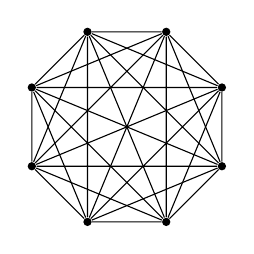
\begin{tikzpicture}

    \node [circ] (0) at (1, 0) {};
    \node [circ] (1) at (0, 0) {};
    \node [circ] (2) at (-0.707, -0.707) {};
    \node [circ] (3) at (-0.707, -1.707) {};
    \node [circ] (4) at (0, -2.414) {};
    \node [circ] (5) at (1, -2.414) {};
    \node [circ] (6) at (1.707, -1.707) {};
    \node [circ] (7) at (1.707, -0.707) {};

    \draw (0) -- (1) -- (2) -- (3) -- (4) -- (5) -- (6) -- (7) -- (0);
    \draw (0) -- (2) -- (4) -- (6) -- (0);
    \draw (1) -- (3) -- (5) -- (7) -- (1);
    \draw (0) -- (3) -- (6) -- (1) -- (4) -- (7) -- (2) -- (5) -- (0);
    \draw (0) -- (4);
    \draw (1) -- (5);
    \draw (2) -- (6);
    \draw (3) -- (7);
  \end{tikzpicture}
\end{center}
We then colour each edge with either red or blue:
\begin{center}
  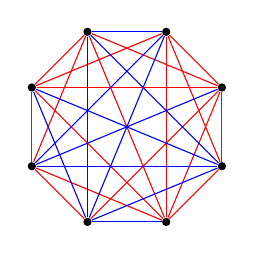
\begin{tikzpicture}

    \node [circ] (0) at (1, 0) {};
    \node [circ] (1) at (0, 0) {};
    \node [circ] (2) at (-0.707, -0.707) {};
    \node [circ] (3) at (-0.707, -1.707) {};
    \node [circ] (4) at (0, -2.414) {};
    \node [circ] (5) at (1, -2.414) {};
    \node [circ] (6) at (1.707, -1.707) {};
    \node [circ] (7) at (1.707, -0.707) {};

    \draw [red] (3) -- (4);
    \draw [red] (5) -- (0);
    \draw [red] (5) -- (6);
    \draw [red] (1) -- (5);
    \draw [red] (0) -- (2);
    \draw [red] (1) -- (3);
    \draw [red] (3) -- (5);
    \draw [red] (2) -- (5);
    \draw [red] (5) -- (7);
    \draw [red] (1) -- (2);
    \draw [red] (7) -- (2);
    \draw [red] (2) -- (3);
    \draw [red] (6) -- (0);
    \draw [red] (7) -- (0);
    \draw [red] (6) -- (7);
    \draw [red] (7) -- (1);
    \draw [red] (4) -- (7);
    \draw [blue] (0) -- (1);
    \draw [blue] (1) -- (4);
    \draw [blue] (2) -- (4);
    \draw [blue] (0) -- (4);
    \draw [blue] (3) -- (7);
    \draw [blue] (4) -- (5);
    \draw [blue] (6) -- (1);
    \draw [blue] (3) -- (6);
    \draw [blue] (0) -- (3);
    \draw [blue] (2) -- (6);
    \draw [blue] (4) -- (6);
  \end{tikzpicture}
\end{center}
We now try to find a (complete) \emph{subgraph} that is monochromatic, i.e.\ a subgraph all of whose edges are the same colour. With a bit of effort, we can find a red monochromatic subgraph of size $4$:
\begin{center}
  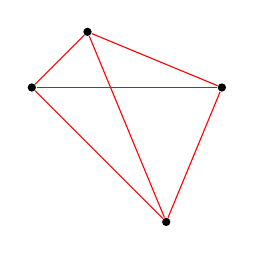
\begin{tikzpicture}

    \node [circ] (1) at (0, 0) {};
    \node [circ] (2) at (-0.707, -0.707) {};
    \node [circ] (5) at (1, -2.414) {};
    \node [circ] (7) at (1.707, -0.707) {};

    \draw [red] (1) -- (5);
    \draw [red] (2) -- (5);
    \draw [red] (5) -- (7);
    \draw [red] (1) -- (2);
    \draw [red] (7) -- (2);
    \draw [red] (7) -- (1);
  \end{tikzpicture}
\end{center}
Are we always guaranteed that we can find a monochromatic subgraph of size $4$? If not, how big does the initial graph have to be? These are questions we will answer in this course. Often, we will ask the question in an ``infinite'' form --- given an \emph{infinite} graph, is it always possible to find an infinite monochromatic subgraph? The answer is yes, and it turns out we can deduce results about the finitary version just by knowing the infinite version.

These questions about graphs will take up the first chapter of the course. In the remaining of the course, we will discuss Ramsey theory on the integers, which, for the purpose of this course, will always mean $\N = \{1, 2, 3, \cdots\}$. We will now try to answer questions about the \emph{arithmetic structure} of $\N$. For example, when we finitely colour $\N$, can we find an infinite arithmetic progression? With some thought, we can see that the answer is no. However, it turns out we can find arbitrarily long arithmetic progressions.

More generally, suppose we have some system of linear equations
\begin{align*}
  3x + 6y + 2z &= 0\\
  2x + 7y + 3z &= 0.
\end{align*}
If we finitely colour $\N$, can we always find a monochromatic solution to these equations?

Remarkably, there is a \emph{complete characterization} of all linear systems that always admit monochromatic solutions. This is given by \emph{Rado's theorem}, which is one of the hardest theorems we are going to prove in the course.

If we are brave, then we can try to get the multiplicative structure of $\N$ in the picture. We begin by asking the most naive question --- if we finitely colour $\N$, can we always find $x, y \in \N$, not both $2$, such that $x + y$ and $xy$ are the same colour? This is a very hard question, and the answer turns out to be yes.

\section{Graph Ramsey theory}
\subsection{Infinite graphs}
We begin by laying out some notations and definitions.
\begin{defi}[$\N$ and $\lbrack n\rbrack$]\index{$\N$}\index{$[n]$}
  We write
  \[
    \N = \{1, 2, 3, 4, \cdots\}.
  \]
  We also write
  \[
    [n] = \{1, 2, 3, \cdots, n\}.
  \]
\end{defi}

\begin{notation}
  For a set $X$, we write $X^{(r)}$\index{$X^{(r)}$} for the subsets of $X$ of size $r$. The elements are known as \term{$r$-sets}.
\end{notation}

We all know what a graph is, hopefully, but for concreteness we provide a definition:
\begin{defi}[Graph]\index{graph}
  A graph $G$ is a pair $(V, E)$, where $E \subseteq V^{(2)}$.
\end{defi}
In particular, our graphs are not directed.

We are mostly interested in graphs with $V = \N$ or $[n]$. In this case, we will write an edge $\{i, j\}$ as $ij$, and always assume that $i < j$. More generally, in $\N^{(r)}$, we write $i_1 i_2 \cdots i_r$ for an $r$-set, and implicitly assume $i_1 < i_2 < \cdots < i_r$.

\begin{defi}[$k$-colouring]\index{$k$-colouring}\index{colouring}
  A $k$-colouring of a set $X$ is a map $c: X \to [k]$.
\end{defi}
Of course, we often replace $k$ with some actual set of colours, e.g.\ $\{\mathrm{red}, \mathrm{blue}\}$. We make more obvious definitions:

\begin{defi}[Monochromatic set]\index{monochromatic set}
  Let $X$ be a set with a $k$-colouring. We say a subset $Y \subseteq X$ is \emph{monochromatic} if the colouring restricted to $Y$ is constant.
\end{defi}

The first question we are interested is in the following --- if $\N^{(2)}$ is $k$-coloured, can we find a complete infinite subgraph that is monochromatic? In other words, is there an infinite subset $X \subseteq \N$ such that $X^{(2)} \subseteq \N^{(2)}$ is monochromatic?

We begin by trying some examples. The correct way to read these examples is to stare at the colouring, and then try to find a monochromatic subset yourself, instead of immediately reading on to see what the monochromatic subset is.
\begin{eg}
  Suppose we had the colouring $c: \N^{(2)} \to \{\mathrm{red}, \mathrm{blue}\}$ by
  \[
    c(ij) =
    \begin{cases}
      \mathrm{red} & i + j \text{ is even}\\
      \mathrm{blue} & i + j \text{ is odd}
    \end{cases}.
  \]
  Then we can pick $X = \{2, 4, 6, 8, \cdots \}$, and this is an infinite monochromatic set.
\end{eg}

\begin{eg}
  Consider $c: \N^{(2)} \to \{0, 1, 2\}$, where
  \[
    c(ij) = \max \{n: 2^n \mid i + j\} \bmod 3
  \]
  In this case, taking $X = \{8, 8^2, 8^3, \cdots\}$ gives an infinite monochromatic set of colour $0$.
\end{eg}

\begin{eg}
  Let $c: \N^{(2)} \to \{\mathrm{red}, \mathrm{blue}\}$ by
  \[
    c(ij) =
    \begin{cases}
      \mathrm{red} & i + j\text{ has an even number of distinct prime factors}\\
      \mathrm{blue} & \mathrm{otherwise}
    \end{cases}
  \]
\end{eg}
It is in fact an open problem to find an explicit infinite monochromatic set for this colouring, or even for which colour do we have an infinite monochromatic set. However, we can prove that such a set must exist!

\begin{thm}[Ramsey's theorem]\index{Ramsey's theorem}
  Whenever we $k$-colour $\N^{(2)}$, there exists an infinite monochromatic set $X$, i.e.\ given any map $c: \N^{(2)} \to [k]$, there exists a subset $X \subseteq \N$ such that $X$ is infinite and $c|_{X^{(2)}}$ is a constant function.
\end{thm}

\begin{proof}
  Pick an arbitrary point $a_1 \in \N$. Then by the pigeonhole principle, there must exist an infinite set $\mathcal{B}_1 \subseteq \N \setminus \{a_1\}$ such that all the $a_1\mdash \mathcal{B}_1$ edges (i.e.\ edges of the form $(a_1, b_1)$ with $b_1 \in \mathcal{B}_1$) are of the same colour $c_1$.

  Now again arbitrarily pick an element $a_2 \in \mathcal{B}_1$. Again, we find some infinite $\mathcal{B}_2 \subseteq \mathcal{B}_1$ such that all $a_2$-$\mathcal{B}_2$ edges are the same colour $c_2$. We proceed inductively.
  \begin{center}
    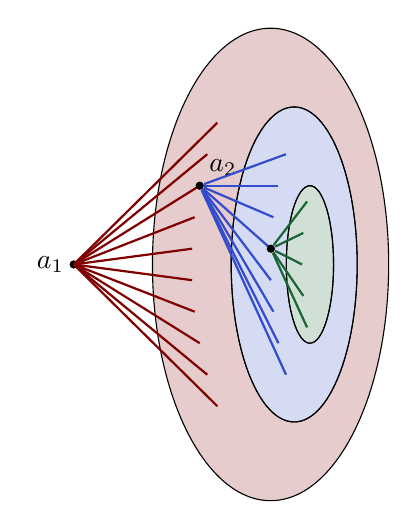
\begin{tikzpicture}
      \draw [fill opacity=0.2, fill=mred] ellipse (1.5 and 3);

      \draw [fill=white] (0.3, 0) ellipse (0.8 and 2);
      \draw [fill opacity=0.2, fill=mblue] (0.3, 0) ellipse (0.8 and 2);
      \draw [fill=white] (0.5, 0) ellipse (0.3 and 1);
      \draw [fill opacity=0.2, fill=mgreen] (0.5, 0) ellipse (0.3 and 1);

      \node [circ] at (-2.5, 0) {};
      \node [left] at (-2.5, 0) {$a_1$};

      \foreach \y in {1.8, 1.4, 1, 0.6, 0.2, -0.2, -0.6, -1, -1.4, -1.8} {
        \pgfmathsetmacro{\x}{-1 + 0.1 * abs(\y)^2};
        \draw [mred, thick] (-2.5, 0) -- (\x, \y) ;
      }
      \node [circ] (a2) at (-0.9, 1) {};
      \node [anchor=south west] at (a2) {$a_2$};
      \foreach \y in {1.4, 1, 0.6, 0.2, -0.2, -0.6, -1, -1.4} {
        \pgfmathsetmacro{\x}{0.1 * abs(\y)^2};
        \draw [mblue, thick] (a2) -- (\x, \y) ;
      }
      \node [circ] (a3) at (0.004, 0.2) {};
      \foreach \y in {0.8, 0.4, 0, -0.4, -0.8} {
        \pgfmathsetmacro{\x}{0.4 + 0.1 * abs(\y)^2};
        \draw [mgreen, thick] (a3) -- (\x, \y) ;
      }
    \end{tikzpicture}
  \end{center}
  We obtain a sequence $\{a_1, a_2, \cdots\}$ and a sequence of colours $\{c_1, c_2, \cdots\}$ such that $c(a_i, a_j) = c_i$, for $i < j$.

  Now again by the pigeonhole principle, since there are finitely many colours, there exists an infinite subsequence $c_{i_1}, c_{i_2}, \cdots$ that is constant. Then $a_{i_1}, a_{i_2}, \cdots$ is an infinite monochromatic set, since all edges are of the colour $c_{i_1} = c_{i_2} = \cdots$. So we are done.
\end{proof}
This proof exhibits many common themes we will see in the different Ramsey theory proofs we will later do. The first is that the proof is highly non-constructive. Not only does it not give us the infinite monochromatic set; it doesn't even tell us what the colour is.

Another feature of the proof is that we did not obtain the infinite monochromatic set in one go. Instead, we had to first pass through that intermediate structure, and then obtain an infinite monochromatic set from that. In future proofs, we might have to go through \emph{many} passes, instead of just two.

This theorem looks rather innocuous, but it has many interesting applications.
\begin{cor}[Bolzano-Weierstrass theorem]
  Let $(x_i)_{i \geq 0}$ be a bounded sequence of real numbers. Then it has a convergent subsequence.
\end{cor}

\begin{proof}
  We define a colouring $c: \N^{(2)} \to \{\uparrow, \downarrow\}$, where
  \[
    c(ij) =
    \begin{cases}
      \uparrow & x_i < x_j\\
      \downarrow & x_j \leq x_i
    \end{cases}
  \]
  Then Ramsey's theorem gives us an infinite monochromatic set, which is the same as a monotone subsequence. Since this is bounded, it must convergence.
\end{proof}

With a very similar technique, we can prove that we can do this for $\N^{(r)}$ for any $r$, and not just $\N^{(2)}$.
\begin{thm}[Ramsey's theorem for $r$ sets]\index{Ramsey's theorem!for $r$ sets}
  Whenever $\N^{(r)}$ is $k$-coloured, there exists an infinite monochromatic set, i.e.\ for any $c: \N^{(r)} \to [k]$, there exists an infinite $X \subseteq \N$ such that $c|_{X^{(r)}}$ is constant.
\end{thm}

We can again try some concrete examples:
\begin{eg}
  We define $c: \N^{(3)} \to \{\mathrm{red}, \mathrm{blue}\}$ by
  \[
    c(ijk) =
    \begin{cases}
      \mathrm{red} & i \mid j + k\\
      \mathrm{blue} & \mathrm{otherwise}
    \end{cases}
  \]
  Then $X = \{2^0, 2^1, 2^2, \cdots\}$ is an infinite monochromatic set.
\end{eg}

\begin{proof}
  We induct on $r$. This is trivial when $r = 1$. Assume $r > 1$. We fix $a_1 \in \N$. We induce a $k$-colouring $c_1$ of $(\N \setminus \{a_1\})^{(r - 1)}$ by
  \[
    c_1(F) = c(F \cup \{a_1\}).
  \]
  By induction, there exists an infinite $B_1 \subseteq \N \setminus \{a_1\}$ such that $B_1$ is monochromatic for $c_1$, i.e.\ all $a_1\mdash B_1$ $r$-sets have the same colour $c_1$.

  We proceed inductively as before. We get $a_1, a_2, a_3, \cdots$ and colours $c_1, c_2, \cdots$ etc. such that for any $r$-set $F$ contained in $\{a_1, a_2, \cdots\}$, we have $c(F) = c_{\min F}$.

  Then again, there exists $c_{i_1}, c_{i_2}, c_{i_3}, \cdots$ all identical, and our monochromatic set is $\{a_{i_1}, a_{i_2}, a_{i_3}, \cdots\}$.
\end{proof}

Now a natural question to ask is --- what happens when we have infinitely many colours? Clearly an infinite monochromatic subset cannot be guaranteed, because we can just colour all edges with different colours.

The natural compromise is to ask if we can find an $X$ such that \emph{either} $c|_{X}$ is monochromatic, \emph{or} $c|_{X}$ is injective. After a little thought, we realize this is also impossible. We can construct a colouring on $\N^{(2)}$ as follows: we first colour all edges that involve $1$ with the colour $1$, then all edges that involve $2$ with the colour $2$ etc:
\begin{center}
  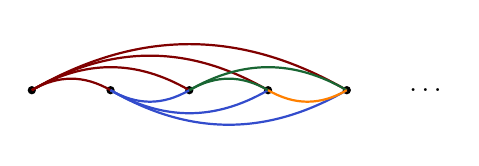
\begin{tikzpicture}
    \foreach \x in {1, 2, 3, 4, 5} {
      \node [circ] at (\x, 0) {};
    }

    \foreach \x in {2, 3, 4, 5} {
      \draw (1, 0) edge [bend left, mred, thick] (\x, 0);
    }
    \foreach \x in {3, 4, 5} {
      \draw (2, 0) edge [bend right, mblue, thick] (\x, 0);
    }
    \foreach \x in {4, 5} {
      \draw (3, 0) edge [bend left, mgreen, thick] (\x, 0);
    }
    \foreach \x in {5} {
      \draw (4, 0) edge [bend right, morange, thick] (\x, 0);
    }
    \node at (6, 0) {$\ldots$};
  \end{tikzpicture}
\end{center}
It is easy to see that we cannot find an infinite monochromatic subset or an infinite subset with all edges of different colours.

However, this counterexample we came up with still has a high amount of structure --- the colour of the edges are uniquely determined by the first element. It turns out this is the only missing piece (plus the obvious dual case).

With this, we can answer our previous question:
\begin{thm}[Canonical Ramsey theorem]\index{canonical Ramsey theorem}\index{Ramsey theorem!canonical}
  For any $c: \N^{(2)} \to \N$, there exists an infinite $X \subseteq \N$ such that one of the following hold:
  \begin{enumerate}
    \item $c|_{X^{(2)}}$ is constant.
    \item $c|_{X^{(2)}}$ is injective.
    \item $c(ij) = c(k\ell)$ iff $i = k$ for all $i, j, k, \ell \in X$.
    \item $c(ij) = c(k\ell)$ iff $j = \ell$ for all $i, j, k, \ell \in X$.
  \end{enumerate}
\end{thm}
Recall that when we write $ij$, we always implicitly assume $i < j$, so that (iii) and (iv) make sense.

In previous proofs, we only had to go through two passes to get the desired set. This time we will need more.
\begin{proof}
  Consider the following colouring of $X^{(4)}$: let $c_1$ be a $2$-colouring
  \[
    c_1(ijk\ell) =
    \begin{cases}
      \mathtt{SAME} & c(ij) = c(k\ell)\\
      \mathtt{DIFF} & \mathrm{otherwise}
    \end{cases}
  \]
  \begin{center}
    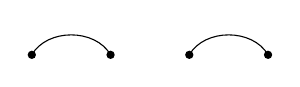
\begin{tikzpicture}
      \foreach \x in {0, 1, 2, 3} {
        \node [circ] at (\x, 0) {};
      }
      \draw (0, 0) edge [out=60, in=120] (1, 0);
      \draw (2, 0) edge [out=60, in=120] (3, 0);
    \end{tikzpicture}
  \end{center}
  Then we know there is some infinite monochromatic set $X_1 \subseteq \N$ for $c_1$. If $X_1$ is coloured $\mathtt{SAME}$, then we are done. Indeed, for any pair $ij$ and $i'j'$ in $X_1$, we can pick some huge $k, \ell$ such that $j, j' < k < \ell$, and then
  \[
    c(ij) = c(k\ell) = c(i'j')
  \]
  as we know $c_1(ijk\ell) = c_1(i'j'k\ell) = \mathtt{SAME}$.

  What if $X_1$ is coloured $\mathtt{DIFF}$? We next look at what happens when we have edges that are nested each other. We define $c_2: X_1^{(4)} \to \{\mathtt{SAME}, \mathtt{DIFF}\}$ defined by
  \[
    c_2(ijk\ell) =
    \begin{cases}
      \mathtt{SAME} & c(i\ell) = c(jk)\\
      \mathtt{DIFF} & \mathrm{otherwise}
    \end{cases}
  \]
  \begin{center}
    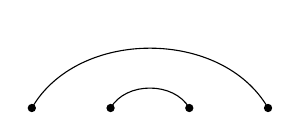
\begin{tikzpicture}
      \foreach \x in {0, 1, 2, 3} {
        \node [circ] at (\x, 0) {};
      }
      \draw (0, 0) edge [out=60, in=120] (3, 0);
      \draw (1, 0) edge [out=60, in=120] (2, 0);
    \end{tikzpicture}
  \end{center}
  Again, we can find an infinite monochromatic subset $X_2 \subseteq X_1$ with respect to $c_2$.

  We now note that $X_2$ cannot be coloured $\mathtt{SAME}$. Indeed, we can just look at
  \begin{center}
    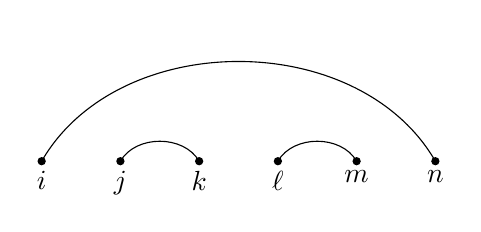
\begin{tikzpicture}
      \foreach \x/\y in {0/i, 1/j, 2/k, 3/\ell, 4/m, 5/n} {
        \node [circ] at (\x, 0) {};
        \node [below] at (\x, 0) {$\y$};
      }
      \draw (0, 0) edge [out=60, in=120] (5, 0);
      \draw (1, 0) edge [out=60, in=120] (2, 0);
      \draw (3, 0) edge [out=60, in=120] (4, 0);
    \end{tikzpicture}
  \end{center}
  So if $X_2$ were $\mathtt{SAME}$, we would have
  \[
    c(\ell m) = c(in) = c(jk),
  \]
  which is impossible since $X_1$ is coloured $\mathtt{DIFF}$ under $c_1$.

  So $X_2$ is $\mathtt{DIFF}$. Now consider $c_3: X_2^{(4)} \to \{\mathtt{SAME}, \mathtt{DIFF}\}$ given by
  \[
    c_3(ijk\ell) =
    \begin{cases}
      \mathtt{SAME} & c(ik) = c(j\ell)\\
      \mathtt{DIFF} & \mathrm{otherwise}
    \end{cases}
  \]
  \begin{center}
    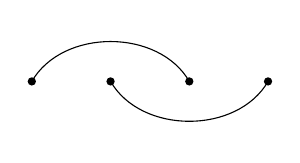
\begin{tikzpicture}
      \foreach \x in {0, 1, 2, 3} {
        \node [circ] at (\x, 0) {};
      }
      \draw (0, 0) edge [out=60, in=120] (2, 0);
      \draw (1, 0) edge [out=-60, in=-120] (3, 0);
    \end{tikzpicture}
  \end{center}
  Again find an infinite monochromatic subset $X_3 \subseteq X_2$ for $c_3$. Then $X_3$ cannot be $\mathtt{SAME}$, this time using the following picture:
   \begin{center}
    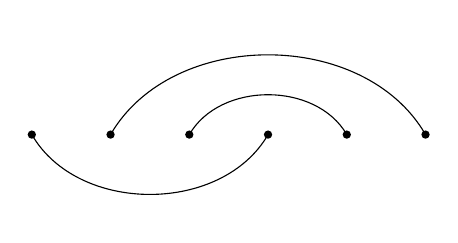
\begin{tikzpicture}
      \foreach \x/\y in {0, 1, 2, 3, 4, 5} {
        \node [circ] at (\x, 0) {};
      }
      \draw (0, 0) edge [out=-60, in=-120] (3, 0);
      \draw (1, 0) edge [out=60, in=120] (5, 0);
      \draw (2, 0) edge [out=60, in=120] (4, 0);
    \end{tikzpicture}
  \end{center}
  contradicting the fact that $c_2$ is $\mathtt{DIFF}$. So we know $X_3$ is $\mathtt{DIFF}$.

  We have now have ended up in this set $X_3$ such that if we have any two pairs of edges with different end points, then they must be different.

  We now want to look at cases where things share a vertex. Consider $c_4: X_3^{(3)} \to \{\mathtt{SAME}, \mathtt{DIFF}\}$ given by
  \[
    c_4(ijk) =
    \begin{cases}
      \mathtt{SAME} & c(ij) = c(jk)\\
      \mathtt{DIFF} & \mathrm{otherwise}
    \end{cases}
  \]
  \begin{center}
    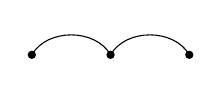
\begin{tikzpicture}
      \foreach \x in {0, 1, 2} {
        \node [circ] at (\x, 0) {};
      }
      \draw (0, 0) edge [out=60, in=120] (1, 0);
      \draw (1, 0) edge [out=60, in=120] (2, 0);
    \end{tikzpicture}
  \end{center}
  Let $X_4 \subseteq X_3$ be an infinite monochromatic set for $c_4$. Now $X_4$ cannot be coloured $\mathtt{SAME}$, using the following picture:
  \begin{center}
    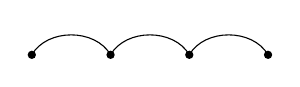
\begin{tikzpicture}
      \foreach \x in {0, 1, 2, 3} {
        \node [circ] at (\x, 0) {};
      }
      \draw (0, 0) edge [out=60, in=120] (1, 0);
      \draw (1, 0) edge [out=60, in=120] (2, 0);
      \draw (2, 0) edge [out=60, in=120] (3, 0);
    \end{tikzpicture}
  \end{center}
  which contradicts the fact that $c_1$ is $\mathtt{DIFF}$. So we know $X_4$ is also coloured $\mathtt{DIFF}$ under $c_4$.

  We are almost there. We need to deal with edges that nest in the sense of (iii) and (iv). We look at $c_5: X_4^{(3)} \to \{\mathtt{LSAME}, \mathtt{LDIFF}\}$ given by
  \[
    c_5(ijk) =
    \begin{cases}
      \mathtt{LSAME} & c(ij) = c(ik)\\
      \mathtt{LDIFF} & \mathrm{otherwise}
    \end{cases}
  \]
   \begin{center}
    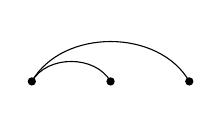
\begin{tikzpicture}
      \foreach \x in {0, 1, 2} {
        \node [circ] at (\x, 0) {};
      }
      \draw (0, 0) edge [out=60, in=120] (1, 0);
      \draw (0, 0) edge [out=60, in=120] (2, 0);
    \end{tikzpicture}
  \end{center}
  Again we find $X_5 \subseteq X_4$, an infinite monochromatic set for $c_5$. We don't separate into cases yet, because we know both cases are possible, but move on to classify the right case as well. Define $c_6: X_5^{(3)} \to \{\mathtt{RSAME}, \mathtt{RDIFF}\}$ given by
  \[
    c_5(ijk) =
    \begin{cases}
      \mathtt{RSAME} & c(ik) = c(jk)\\
      \mathtt{RDIFF} & \mathrm{otherwise}
    \end{cases}
  \]
   \begin{center}
    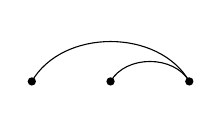
\begin{tikzpicture}
      \foreach \x in {0, 1, 2} {
        \node [circ] at (\x, 0) {};
      }
      \draw (1, 0) edge [out=60, in=120] (2, 0);
      \draw (0, 0) edge [out=60, in=120] (2, 0);
    \end{tikzpicture}
  \end{center}
  Let $X_6 \subseteq X_5$ be an infinite monochromatic subset under $c_5$.

  As before, we can check that it is impossible to get both $\mathtt{LSAME}$ and $\mathtt{RSAME}$, using the following picture:
  \begin{center}
    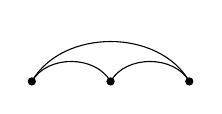
\begin{tikzpicture}
      \foreach \x in {0, 1, 2} {
        \node [circ] at (\x, 0) {};
      }
      \draw (0, 0) edge [out=60, in=120] (1, 0);
      \draw (1, 0) edge [out=60, in=120] (2, 0);
      \draw (0, 0) edge [out=60, in=120] (2, 0);
    \end{tikzpicture}
  \end{center}
  contradicting $c_4$ being $\mathtt{DIFF}$.

  Then the remaining cases $(\mathtt{LDIFF}, \mathtt{RDIFF})$, $(\mathtt{LSAME}, \mathtt{RDIFF})$ and $(\mathtt{RDIFF}, \mathtt{LSAME})$ corresponds to the cases (ii), (iii) and (iv).
\end{proof}
Note that we could this theorem in one pass only, instead of six, by considering a much more complicated colouring $(c_1, c_2, c_3, c_4, c_5, c_6)$ with values in
\[
  \{\mathtt{SAME}, \mathtt{DIFF}\}^4 \times \{\mathtt{LSAME}, \mathtt{LDIFF}\} \times \{\mathtt{RSAME}, \mathtt{RDIFF}\},
\]
but we still have to do the same analysis and it just complicates matters more.

There is a generalization of this to $r$-sets. One way we can rewrite the theorem is to say that the colour is uniquely determined by some subset of the vertices. The cases (i), (ii), (iii), (iv) correspond to no vertices, all vertices, first vertex, and second vertex respectively. Then for $r$-sets, we have $2^r$ possibilities, one for each subset of the $r$-coordinates.

\begin{thm}[Higher dimensional canonical Ramsey theorem]\index{higher dimensional canonical Ramsey theorem}\index{canonical Ramsey theorem!!higher dimensional}\index{Ramsey theorem!higher dimensional, canonical}
  Let $c: \N^{(r)} \to \N$ be a colouring. Then there exists $D \subseteq [r]$ and an infinite subset $X \subseteq \N$ such that for all $x, y \in X^{(r)}$, we have $c(x) = c(y)$ if $\{i: x_i = y_i\} \supseteq D$, where $x = \{x_1 < x_2 < \cdots < x_r\}$ (and similarly for $y$).
\end{thm}

\subsection{Finite graphs}
We now move on to discuss a finitary version of the above problem. Of course, if we finitely colour an infinite graph, then we can obtain a finite monochromatic subgraph of any size we want, because this is just a much weaker version of Ramsey's theorem. However, given $n < N$, if we finitely colour a graph of size $N$, are we guaranteed to have a monochromatic subgraph of size $n$?

Before we begin, we note some definitions. Recall again that a graph $G$ is a pair $(V, E)$ where $E \subseteq V^{(2)}$.
\begin{eg}
  The \term{path graph} on $n$ vertices \term{$P_n$} is
  \begin{center}
    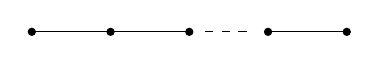
\begin{tikzpicture}
      \draw (0, 0) node [circ] {} -- (1, 0) node [circ] {} -- (2, 0) node [circ] {};

      \draw [dashed] (2.2, 0) -- (2.8, 0);

      \draw (3, 0) node [circ] {} -- (4, 0) node [circ] {};
    \end{tikzpicture}
  \end{center}
  We can write
  \[
    V = [n],\quad E = \{12, 23, 34, \cdots, (n-1)n\}.
  \]
\end{eg}

\begin{eg}
  The $n$-cycle \term{$C_n$} is
  \[
    V = [n],\quad E = \{12, 23, \cdots, (n-1)n, 1n\}.
  \]
  \begin{center}
    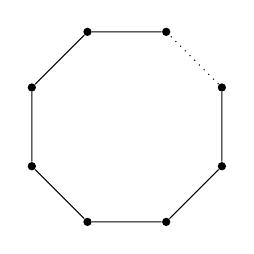
\begin{tikzpicture}

      \node [circ] (0) at (1, 0) {};
      \node [circ] (1) at (0, 0) {};
      \node [circ] (2) at (-0.707, -0.707) {};
      \node [circ] (3) at (-0.707, -1.707) {};
      \node [circ] (4) at (0, -2.414) {};
      \node [circ] (5) at (1, -2.414) {};
      \node [circ] (6) at (1.707, -1.707) {};
      \node [circ] (7) at (1.707, -0.707) {};

      \draw (0) -- (1) -- (2) -- (3) -- (4) -- (5) -- (6) -- (7);
      \draw [dotted] (7) -- (0);
    \end{tikzpicture}
  \end{center}
\end{eg}

Finally, we have
\begin{eg}
  The \term{complete graph} \term{$V_n$} on $n$ vertices is
  \[
    V = [n],\quad E = V^{(2)}.
  \]
  \begin{center}
    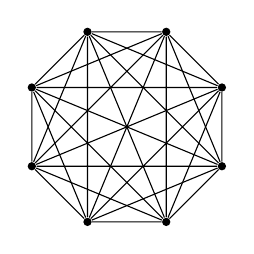
\begin{tikzpicture}

      \node [circ] (0) at (1, 0) {};
      \node [circ] (1) at (0, 0) {};
      \node [circ] (2) at (-0.707, -0.707) {};
      \node [circ] (3) at (-0.707, -1.707) {};
      \node [circ] (4) at (0, -2.414) {};
      \node [circ] (5) at (1, -2.414) {};
      \node [circ] (6) at (1.707, -1.707) {};
      \node [circ] (7) at (1.707, -0.707) {};

      \draw (0) -- (1) -- (2) -- (3) -- (4) -- (5) -- (6) -- (7) -- (0);
      \draw (0) -- (2) -- (4) -- (6) -- (0);
      \draw (1) -- (3) -- (5) -- (7) -- (1);
      \draw (0) -- (3) -- (6) -- (1) -- (4) -- (7) -- (2) -- (5) -- (0);
      \draw (0) -- (4);
      \draw (1) -- (5);
      \draw (2) -- (6);
      \draw (3) -- (7);
    \end{tikzpicture}
  \end{center}
\end{eg}
Concretely, the question we want to answer is the following --- how big does our (complete) graph have to be to guarantee a complete monochromatic subgraph of size $n$?

In this section, we will usually restrict to $2$ colours. Everything we say will either be trivially be generalizable to more colours, or we have no idea how to do so. It is an exercise for the reader to figure out which it is.
\begin{defi}[Ramsey number]\index{Ramsey number}\index{$R(n)$}\index{$R(K_n)$}
  We let $R(n) = R(K_n)$ to be the smallest $N \in \N$ whenever we red-blue colour the edges of $K_N$, then there is a monochromatic copy of $K_n$.
\end{defi}

It is not immediately obvious that $R(n)$ has to exist, i.e.\ it is a finite number. It turns out we can easily prove this from the infinite Ramsey theorem.
\begin{thm}[Finite Ramsey theorem]\index{finite Ramsey theorem}
  For all $n$, we have $R(n) < \infty$.
\end{thm}

\begin{proof}
  Suppose not. Let $n$ be such that $R(n) = \infty$. Then for any $m \geq n$, there is a $2$-colouring $c_m$ of $K_m = [m]^{(2)}$ such that there is no monochromatic set of size $n$.

  We want to use these colourings to build up a colouring of $\N^{(2)}$ with no monochromatic set of size $n$. We want to say we take the ``limit'' of these colourings, but what does this mean? To do so, we need these colourings to be nested.

  By the pigeonhole principle, there exists an infinite set $M_1 \subseteq \N$ and some fixed $2$-colouring $d_n$ of $[n]$ such that $c_m|_{[n]^{(2)}} = d_n$ for all $m \in M_1$.

  Similarly, there exists an infinite $M_2 \subseteq M_1$ such that $c_m|_{[n + 1]^{(2)}} = d_{n + 1}$ for $m \in M_2$, again for some $2$-colouring $d_{n + 1}$ of $[n + 1]$. We repeat this over and over again. Then we get a sequence $d_n, d_{n + 1}, \cdots$ of colourings such that $d_i$ is a $2$-colouring of $[i]^{(2)}$ without a monochromatic $K_n$, and further for $i < j$, we have
  \[
    d_j|_{[i]^{(2)}} = d_i.
  \]
  We then define a $2$-colouring $c$ of $\N^{(2)}$ by
  \[
    c(ij) = d_m(ij)
  \]
  for any $m > i, j$. Clearly, there exists no monochromatic $K_n$ in $c$, as any $K_n$ is finite. This massively contradicts the infinite Ramsey theorem.
\end{proof}

There are other ways of obtaining the finite Ramsey theorem from the infinite one. For example, we can use the compactness theorem for first order logic.
\begin{proof}
  Suppose $R(n) = \infty$. Consider the theory with proposition letters $p_{ij}$ for each $ij \in \N^{(2)}$. We will think of the edge $ij$ as red if $p_{ij} = \top$, and blue if $p_{ij} = \bot$. For each subset of $\N$ of size $n$, we add in the axiom that says that set is not monochromatic.

  Then given any finite subset of the axioms, it mentions only finitely many subsets of $\N$. Suppose it mentions vertices only up to $m \in \N$. Then by assumption, there is a $2$-colouring of $[m]^{(2)}$ with no monochromatic subset of size $n$. So by assigning $p_{ij}$ accordingly (and randomly assigning the remaining ones), we have found a model of this finite subtheory. Thus every finite fragment of the theory is consistent. Hence the original theory is consistent. So there is a model, i.e.\ a colouring of $\N^{(2)}$ with no monochromatic subset.

  This contradicts the infinite Ramsey theorem.
\end{proof}

Similarly, we can do it by compactness of the space $\{1, 2\}^\N$ endowed with metric
\[
  d(f, g) = \frac{1}{2^n}\text{ if } n = \min \{i: f_i \not= g_i\}.
\]
By Tychonoff theorem, we know this is compact, and we can deduce the theorem from this. % how?

While these theorems save work by reusing the infinite Ramsey theorem, it is highly non-constructive. It is useless if we want to obtain an actual bound on $R(n)$. We now go back and see what we did when we proved the infinite Ramsey theorem.

To prove the infinite Ramsey theory, We randomly picked a point $a_1$. Then there are some things that are connected by red to it, and others connected by blue:
\begin{center}
  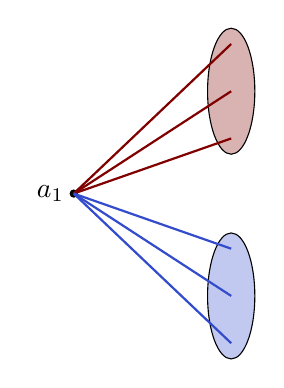
\begin{tikzpicture}
    \node [circ] {};
    \node [left] {$a_1$};

    \draw [fill opacity=0.3, fill=mred] (2, 1.3) ellipse (0.3 and 0.8);
    \draw [fill opacity=0.3, fill=mblue] (2, -1.3) ellipse (0.3 and 0.8);

    \draw [thick, mred] (0, 0) -- (2, 1.9);
    \draw [thick, mred] (0, 0) -- (2, 1.3);
    \draw [thick, mred] (0, 0) -- (2, 0.7);

    \draw [thick, mblue] (0, 0) -- (2, -1.9);
    \draw [thick, mblue] (0, 0) -- (2, -1.3);
    \draw [thick, mblue] (0, 0) -- (2, -0.7);
  \end{tikzpicture}
\end{center}
Next we randomly pick a point in one of the red or blue sets, and try to move on from there. Suppose we landed in the red one. Now note that if we find a blue $K_n$ in the red set, then we are done. But on the other hand, we only need a red $K_{n - 1}$, and not a full blown $K_n$. When we moved to this red set, the problem is no longer symmetric.

Thus, to figure out a good bound, it is natural to consider an asymmetric version of the problem.
\begin{defi}[Off-diagonal Ramsey number]\index{off-diagonal Ramsey number}\index{Ramsey number!off-diagonal}\index{$R(n, m)$}\index{$R(K_n, K_m)$}
  We define $R(n, m) = R(K_n, K_m)$ to be the minimum $N \in \N$ such that whenever we red-blue colour the edges of $K_N$, we either get a red $K_n$ or a blue $K_m$.
\end{defi}

Clearly we have
\[
  R(n, m) \leq R(\max\{n, m\}).
\]
In particular, they are finite. Once we make this definition, it is easy to find a bound on $R$.
\begin{thm}
  We have
  \[
    R(n, m) \leq R(n - 1, m) + R(n, m - 1).
  \]
  for all $n, m \in \N$. Consequently, we have
  \[
    R(n, m) \leq \binom{n + m - 1}{n - 2}.
  \]
\end{thm}

\begin{proof}
  We induct on $n + m$. It is clear that
  \[
    R(1, n) = R(n, 1) = 1,\quad R(n, 2) = R(2, n) = n
  \]
  Now suppose $N \geq R(n - 1, m) + R(n, m - 1)$. Consider any red-blue colouring of $K_N$ and any vertex $v \in V(K_n)$. We write
  \[
    v(K_n) \setminus \{v\} = A \cup B,
  \]
  where each vertex $A$ is joined by a red edge to $v$, and each vertex in $B$ is joined by a blue edge to $v$. Then
  \[
    |A| + |B| \geq N - 1 \geq R(n - 1, m) + R(n, m - 1) - 1.
  \]
  It follows that either $|A| \geq R(n - 1, m)$ or $|B| \geq R(n, m - 1)$. We wlog it is the former. Then by definition of $R(n - 1, m)$, we know $A$ contains either a blue copy of $K_m$ or a red copy of $K_{n - 1}$. In the first case, we are done, and in the second case, we just add $v$ to the red $K_{n - 1}$.

  The last formula is just a straightforward property of binomial coefficients.
\end{proof}

In particular, we find
\[
  R(n) \leq \binom{2n - 1}{n - 2} \leq \frac{4^n}{\sqrt{n}}.
\]
We genuinely have no idea whether $\sim 4^n$ is the correct growth rate, i.e.\ if there is some $\varepsilon$ such that $R(n) \leq (4 - \varepsilon)^n$. However, we do know that for any $c > 0$, we eventually have
\[
  R(n) \leq \frac{4^n}{n^c}.
\]
That was an upper bound. Do we have a lower bound? In particular, does $R(n)$ have to grow exponentially? The answer is yes, and the answer is a very classical construction of Erd\"os.

\begin{thm}
  We have $R(n) \geq \sqrt{2}^n$ for sufficiently large $n \in \N$.
\end{thm}
The proof is remarkable in that before this was shown, we had no sensible bound at all. However, the proof is incredibly simple, and revolutionized how we think about colourings.

\begin{proof}
  Let $N \leq \sqrt{2}^n$. We perform a red-blue colouring of $K_N$ randomly, where each edge is coloured red independently of the others with probability $\frac{1}{2}$.

  We let $X_R$ be the number of red copies of $K_n$ in such a colouring. Then since expectation is linear, we know the expected value is
  \begin{align*}
    [X_R] &= \binom{N}{n} \left(\frac{1}{2}\right)^{\binom{n}{2}}\\
    &\leq \left(\frac{eN}{n}\right)^n \left(\frac{1}{2}\right)^{\binom{n}{2}}\\
    &\leq \left(\frac{e}{n}\right)^n \sqrt{2}^{n^2} \sqrt{2}^{-n^2}\\
    &= \left(\frac{e}{n}\right)^{n}\\
    &< \frac{1}{2}
  \end{align*}
  for sufficiently large $n$.

  Similarly, we have $[X_B] < \frac{1}{2}$. So the expected number of monochromatic $K_n$ is $< 1$. So in particular there must be some colouring with no monochromatic $K_n$.
\end{proof}

Recall the bound
\[
  R(m, n) \leq \binom{m + n - 2}{m - 1}.
\]
If we think of $m$ as being fixed, then this tells us
\[
  R(m, n) \sim (n + m)^{m - 1}.
\]
For example, if $m$ is $3$, then we have
\[
  R(3, n) \leq \binom{n + 1}{2} = \frac{n(n + 1)}{2} \sim n^2.
\]
We can sort-of imagine where this bound came from. Suppose we randomly pick a vertex $v_1$. Then if it is connected to at least $n$ other vertices by a red edge, then we are done --- if there is even one red edge among those $n$ things, then we have a red triangle. Otherwise, all edges are blue, and we've found a complete blue $K_n$.

So this is connected to at most $n - 1$ things by a red edge. So if our graph is big enough, we can pick some $v_2$ connected to $v_1$ by a blue edge, and do the same thing to $v_2$. We keep going on, and by the time we reach $v_n$, we would have found $v_1, \cdots, v_n$ all connected to each other by blue edges, and we are done. So we have $K(3, n) \sim n^2$.
\begin{center}
  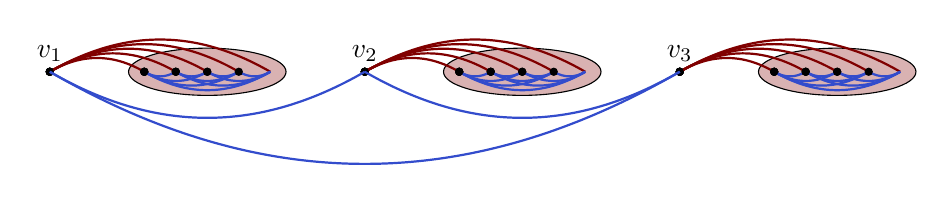
\begin{tikzpicture}
    \foreach \s in {0, 4, 8} {
      \begin{scope}[shift={(\s, 0)}]
        \node [circ] {};

        \draw [fill opacity=0.3, fill=mred] (2, 0) ellipse (1 and 0.3);
        \foreach \x in {1.2,1.6,2.0,2.4,2.8} {
          \draw (0, 0) edge [bend left, mred, thick] (\x, 0) node [circ] {};
        }
        \foreach \x in {1.6,2.0,2.4,2.8} {
          \draw (1.2, 0) edge [bend right, mblue, thick] (\x, 0) node [circ] {};
        }
        \foreach \x in {2.0,2.4,2.8} {
          \draw (1.6, 0) edge [bend right, mblue, thick] (\x, 0) node [circ] {};
        }
        \foreach \x in {2.4,2.8} {
          \draw (2.0, 0) edge [bend right, mblue, thick] (\x, 0) node [circ] {};
        }
        \foreach \x in {2.8} {
          \draw (2.4, 0) edge [bend right, mblue, thick] (\x, 0) node [circ] {};
        }
      \end{scope};
    }
    \draw (0, 0) edge [bend right, mblue, thick] (4, 0);
    \draw (4, 0) edge [bend right, mblue, thick] (8, 0);
    \draw (0, 0) edge [bend right, mblue, thick] (8, 0);
    \node at (0, 0) [above] {$v_1$};
    \node at (4, 0) [above] {$v_2$};
    \node at (8, 0) [above] {$v_3$};
  \end{tikzpicture}
\end{center}
But this argument is rather weak, because we didn't use that large pool of blue edges we've found at $v_1$. So in fact this time we can do better than $n^2$.
\begin{thm}
  We have
  \[
    R(3, n) \leq \frac{100 n^2}{\log n}
  \]
  for sufficiently large $n \in \N$.
\end{thm}
Here the $100$ is, obviously, just some random big number.

\begin{proof}
  Let $N \geq 100n^2/\log n$, and consider a red-blue colouring of the edges of $K_N$ with no red $K_3$. We want to find a blue $K_n$ in such a colouring.

  We may assume that
  \begin{enumerate}
    \item No vertex $v$ has $ \geq n$ red edges incident to it, as argued just now.
    \item If we have $v_1, v_2, v_3$ such that $v_1v_2$ and $v_1 v_3$ are red, then $v_2 v_3$ is blue:
      \begin{center}
        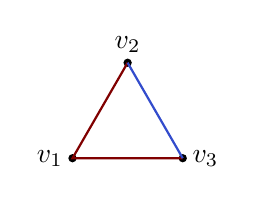
\begin{tikzpicture}[scale=0.7]
          \node [circ] at (0, 0) {};
          \node [circ] at (2, 0) {};
          \node [circ] at (1, 1.732) {};
          \draw [mred, thick] (2, 0) -- (0, 0) -- (1, 1.732);
          \draw [mblue, thick] (1, 1.732) -- (2, 0);

          \node [left] at (0, 0) {$v_1$};
          \node [above] at (1, 1.732) {$v_2$};
          \node [right] at (2, 0) {$v_3$};
        \end{tikzpicture}
      \end{center}
  \end{enumerate}
  We now let
  \[
    \mathcal{F} = \{W : W \subseteq V(K_N)\text{ such that }W^{(2)} \text{ is monochromatic and blue}\}.
  \]
  We want to find some $W \in \mathcal{F}$ such that $|W| \geq n$, i.e.\ a blue $K_n$. How can we go about finding this?

  Let $W$ be a uniformly random member of $\mathcal{F}$. We will be done if we can show that that $\E[|W|] \geq n$.

  We are going to define a bunch of random variables. For each vertex $v \in V(K_N)$, we define the variable
  \[
    X_v = n \mathbf{1}_{\{v \in W\}} + |\{u: uv\text{ is red and }u \in W\}|.
  \]
  \begin{claim}
   \[
    \E[X_v] > \frac{\log n}{10}
  \]
  for each vertex $v$.
  \end{claim}
  To see this, let
  \[
    A = \{u: uv \text{ is red}\}
  \]
  and let
  \[
    B = \{u: uv \text{ is blue}\}.
  \]
  then from the properties we've noted down, we know that $|A| < n$ and $A^{(2)}$ is blue. So we know very well what is happening in $A$, and nothing about what is in $B$.

  We fix a set $S \subseteq B$ such that $S \in \mathcal{F}$, i.e.\ $S^{(2)}$ is blue. What can we say about $W$ if we condition on $B \cap W = S$?
  \begin{center}
    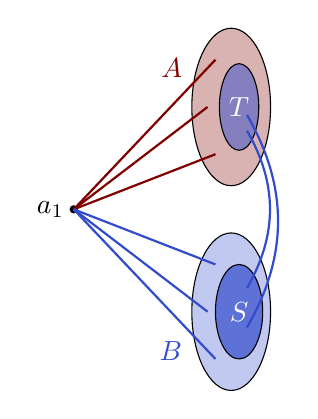
\begin{tikzpicture}
      \node [circ] {};
      \node [left] {$a_1$};

      \draw [fill opacity=0.3, fill=mred] (2, 1.3) ellipse (0.5 and 1);
      \draw [fill opacity=0.3, fill=mblue] (2, -1.3) ellipse (0.5 and 1);

      \draw [thick, mred] (0, 0) -- (1.8, 1.9);
      \draw [thick, mred] (0, 0) -- (1.7, 1.3);
      \draw [thick, mred] (0, 0) -- (1.8, 0.7);

      \draw [thick, mblue] (0, 0) -- (1.8, -1.9);
      \draw [thick, mblue] (0, 0) -- (1.7, -1.3);
      \draw [thick, mblue] (0, 0) -- (1.8, -0.7);

      \draw [fill=mblue, fill opacity=0.7] (2.1, -1.3) ellipse (0.3 and 0.6);

      \node at (2.1, -1.3) [white] {$S$};

      \node [mblue, left] at (1.5, -1.8) {$B$};
      \node [mred, left] at (1.5, 1.8) {$A$};

      \draw [fill=mblue, fill opacity=0.5] (2.1, 1.3) ellipse (0.25 and 0.55);

      \node at (2.1, 1.3) [white] {$T$};

      \draw (2.2, -1) edge [bend right, mblue, thick] (2.2, 1);
      \draw (2.2, -1.5) edge [bend right, mblue, thick] (2.2, 1.2);
    \end{tikzpicture}
  \end{center}
  Let $T \subseteq A$ be the set of vertices that are joined to $S$ only by blue edges. Write $|T| = x$. Then if $B \cap W = S$, then either $W \subseteq S \cup T$, or $W \subseteq S \cup \{v\}$. So there are exactly $2^x + 1$ choices of $W$. So we know
  \begin{align*}
    \E[X_v \mid W \cap B = S] &\geq \frac{n}{2^x + 1} + \frac{2^x}{2^x + 1}(\E[|\text{random subset of T}|])\\
    &= \frac{n}{2^x + 1} + \frac{2^{x - 1}x}{2^x + 1}.
  \end{align*}
  Now if
  \[
    x < \frac{\log n}{2},
  \]
  then
  \[
    \frac{n}{2^x + 1} \geq \frac{n}{\sqrt{n} + 1} \geq \frac{\log n}{10}
  \]
  for all sufficiently large $n$. On the other hand, if
  \[
    x \geq \frac{\log n}{2},
  \]
  then
  \[
    \frac{2^{x - 1}x}{2^x + 1} \geq \frac{1}{4} \cdot \frac{\log n}{2} \geq \frac{\log n}{10}.
  \]
  So we are done.

  \begin{claim}
    \[
      \sum_{v \in V} X_v \leq 2n |W|.
    \]
  \end{claim}
  To see this, for each vertex $v$, we know that if $v \in W$, then it contributes $n$ to the sum via the first term. Also, by our initial observation, we know that $v \in W$ has at most $n$ neighbours. So it contributes at most $n$ to the second term (acting as the ``$u$'').

  Finally, we know that
  \[
    \E[|W|] \geq \frac{1}{2n} \sum \E[X_V] \geq \frac{N}{2n} \frac{\log n}{10} \geq \frac{100n^2}{\log n} \cdot \frac{\log n}{20 n} \geq 5n.
  \]
  Therefore we can always find some $W \in \mathcal{F}$ such that $|W| \geq n$.
\end{proof}

Now of course, there is the following obvious generalization of Ramsey numbers:
\begin{defi}[$R(G, H)$]\index{$R(G, H)$}
  Let $G, H$ be graphs. Then we define $R(G, H)$ to be the smallest $N$ such that any red-blue colouring of $K_N$ has either a red copy of $G$ or a blue copy of $H$.
\end{defi}
Obviously, we have $R(G, H) \leq R(|G|, |H|)$. So the natural question is if we can do better than that.

\begin{ex}
  Show that
  \[
    R(P_n, P_n) \leq 2n.
  \]
\end{ex}
So sometimes it can be much better.

\section{Ramsey theory on the integers}
So far, we've been talking about what happens when we finitely colour graphs. What if we $k$-colour the integers $\N$? What can we say about it?

It is a trivial statement that this colouring has a monochromatic subset, by the pigeonhole principle. Interesting questions arise when we try to take the additive structure of $\N$ into account. So we could ask, can we find a monochromatic ``copy'' of $\N$.

One way to make this question concrete is to ask if there is an infinite monochromatic arithmetic progression.

The answer is easily a ``no''! There are only countably many progressions, so for each arithmetic progression, we pick two things in the progression and colour them differently.

We can also construct this more concretely. We can colour the first number red, the next two blue, the next three red etc. then it is easy to see that it doesn't have an infinite arithmetic progression.
\begin{center}
  \begin{tikzpicture}[xscale=0.5]
    \foreach \x in {0, 3, 4, 5, 10, 11, 12, 13,14} {
      \node [circ, mred] at (\x, 0) {};
    }
    \foreach \x in {1,2,6,7,8,9,15,16,17,18,19,20} {
      \node [circ, mblue] at (\x, 0) {};
    }
    \node at (21.3, 0) {$\cdots$};
  \end{tikzpicture}
\end{center}
But this is somewhat silly, because there is clearly a significant amount of structure in the sequence there. It turns out the following is true:
\begin{thm}[van der Waerden theorem]\index{van der Waerden theorem}
  Let $m, k \in N$. Then there is some $N = W(m, k)$ such that whenever $[N]$ is $k$-coloured, then there is a monochromatic arithmetic progression of length $n$.
\end{thm}

The idea is to do induction on $m$. We will be using colourings with much greater than $k$ colours to deduce the existence of $W(m, k)$.

We can try a toy example first. Let's try to show that $W(3, 2)$ exists. Suppose we have three natural numbers:
\begin{center}
  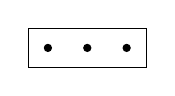
\begin{tikzpicture}[scale=0.5]
    \draw (-0.5, 0.5) rectangle (2.5, -0.5);
    \node [circ] at (0, 0) {};
    \node [circ] at (1, 0) {};
    \node [circ] at (2, 0) {};
  \end{tikzpicture}
\end{center}
By the pigeonhole principle, there must be two things that are the same colour, say
\begin{center}
  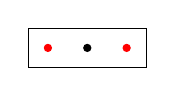
\begin{tikzpicture}[scale=0.5]
    \draw (-0.5, 0.5) rectangle (2.5, -0.5);
    \node [circ, red] at (0, 0) {};
    \node [circ] at (1, 0) {};
    \node [circ, red] at (2, 0) {};
  \end{tikzpicture}
\end{center}
If this is the case, then if we don't want to have an arithmetic progression of length $3$, then the fifth number must be blue
\begin{center}
  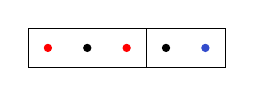
\begin{tikzpicture}[scale=0.5]
    \draw (-0.5, 0.5) rectangle (2.5, -0.5);
    \node [circ, red] at (0, 0) {};
    \node [circ] at (1, 0) {};
    \node [circ, red] at (2, 0) {};

    \draw (2.5, -0.5) rectangle (4.5, 0.5);
    \node [circ] at (3, 0) {};
    \node [circ, mblue] at (4, 0) {};
  \end{tikzpicture}
\end{center}
We now cut the universe into blocks into 5 things. Again by the pigeonhole principle, there must be two blocks that look the same. Say it's this block again.
\begin{center}
  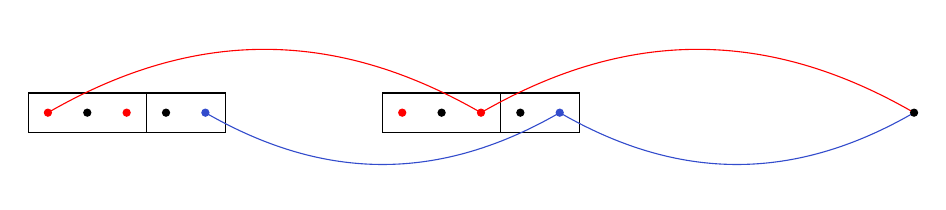
\begin{tikzpicture}[scale=0.5]
    \draw (-0.5, 0.5) rectangle (2.5, -0.5);
    \node [circ, red] at (0, 0) {};
    \node [circ] at (1, 0) {};
    \node [circ, red] at (2, 0) {};

    \draw (2.5, -0.5) rectangle (4.5, 0.5);
    \node [circ] at (3, 0) {};
    \node [circ, mblue] at (4, 0) {};

    \begin{scope}[shift={(9, 0)}]
      \draw (-0.5, 0.5) rectangle (2.5, -0.5);
      \node [circ, red] at (0, 0) {};
      \node [circ] at (1, 0) {};
      \node [circ, red] at (2, 0) {};

      \draw (2.5, -0.5) rectangle (4.5, 0.5);
      \node [circ] at (3, 0) {};
      \node [circ, mblue] at (4, 0) {};
    \end{scope}
    \draw [red] (0, 0) edge [bend left] (11, 0);
    \draw [red] (11, 0) edge [bend left] (22, 0);

    \draw [mblue] (4, 0) edge [bend right] (13, 0);
    \draw [mblue] (13, 0) edge [bend right] (22, 0);

    \node [circ] at (22, 0) {};
  \end{tikzpicture}
\end{center}
Now we have two sequences, and the point at the end belongs to both of the two sequences. And no matter what colour it is, we are done.

For $k = 3$, we can still find such a block, but now that third point could be a third colour, say, green. This will not stop us. We can now look at these big blocks, and we know that eventually, these big blocks must repeat themselves.
\begin{center}
  \begin{tikzpicture}[scale=1.1]
    \draw (-0.05, 0.05) rectangle (0.25, -0.05);
    \node [scirc, red] at (0, 0) {};
    \node [scirc] at (0.1, 0) {};
    \node [scirc, red] at (0.2, 0) {};

    \draw (0.25, -0.05) rectangle (.45, .05);
    \node [scirc] at (.3, 0) {};
    \node [scirc, mblue] at (.4, 0) {};

    \begin{scope}[shift={(.9, 0)}]
      \draw (-.05, .05) rectangle (.25, -.05);
      \node [scirc, red] at (0, 0) {};
      \node [scirc] at (.1, 0) {};
      \node [scirc, red] at (.2, 0) {};

      \draw (.25, -.05) rectangle (.45, .05);
      \node [scirc] at (.3, 0) {};
      \node [scirc, mblue] at (.4, 0) {};
    \end{scope}
    \draw [red] (0, 0) edge [bend left] (5.1, 0);
    \draw [red] (5.1, 0) edge [bend left] (10.2, 0);

    \draw [mblue] (.4, 0) edge [bend right] (5.3, 0);
    \draw [mblue] (5.3, 0) edge [bend right] (10.2, 0);

    \draw [mgreen] (2.2, 0) edge [bend right] (6.2, 0);
    \draw [mgreen] (6.2, 0) edge [bend right] (10.2, 0);

    \node [mgreen, scirc] at (2.2, 0) {};

    \begin{scope}[shift={(4, 0)}]
      \draw (-.05, .05) rectangle (.25, -.05);
      \node [scirc, red] at (0, 0) {};
      \node [scirc] at (.1, 0) {};
      \node [scirc, red] at (.2, 0) {};

      \draw (.25, -.05) rectangle (.45, .05);
      \node [scirc] at (.3, 0) {};
      \node [scirc, mblue] at (.4, 0) {};

      \begin{scope}[shift={(.9, 0)}]
        \draw (-.05, .05) rectangle (.25, -.05);
        \node [scirc, red] at (0, 0) {};
        \node [scirc] at (.1, 0) {};
        \node [scirc, red] at (.2, 0) {};

        \draw (.25, -.05) rectangle (.45, .05);
        \node [scirc] at (.3, 0) {};
        \node [scirc, mblue] at (.4, 0) {};
      \end{scope}

      \node [mgreen, scirc] at (2.2, 0) {};
    \end{scope}

    \node [scirc] at (10.2, 0) {};
  \end{tikzpicture}
\end{center}
Here we did the case $m = 2$, and we used the pigeonhole principle. When we do $m > 2$, we will use van der Waerden theorem for smaller $m$ inductively.

We now come up with names to describe the scenario we had above.
\begin{defi}[Focused progression]\index{focused progression}
  We say a collection of arithmetic progressions $A_1, A_2, \cdots, A_r$ of length $m$ with
  \[
    A_i = \{a_i, a_i + d_i, \cdots, a_i + (m - 1) d_i\}
  \]
  are \emph{focused} at $f$ if $a_i + m d_i = f$ for all $1 \leq i \leq r$.
\end{defi}

\begin{eg}
  $\{1, 4\}$ and $\{5, 6\}$ are focused at $7$.
\end{eg}

\begin{defi}[Colour focused progression]\index{colour focused progression}\index{focus progression!colour}
  If $A_1, \cdots, A_r$ are focused at $f$, and each $A_i$ is monochromatic and no two are the same colour, then we say they are \emph{colour focused} at $f$.
\end{defi}

We can now write the proof.
\begin{proof}
  We induct on $m$. The result is clearly trivial when $m = 1$, and follows easily from the pigeonhole principle when $m = 2$.

  Suppose $m > 1$, and assume inductively that $W(m - 1, k')$ exists for any $k' \in \N$.

  Here is the claim we are trying to established:
  \begin{claim}
    For each $r \leq k$, there is a natural number $n$ such that whenever we $k$-colour $[n]$, then either
    \begin{enumerate}
      \item There exists a monochromatic AP of length $m$; or
      \item There are $r$ colour-focused AP's of length $m - 1$.
    \end{enumerate}
  \end{claim}
  It is clear that this claim implies the theorem, as we can pick $r = k$. Then if there isn't a monochromatic AP of length $m$, then we look at the colour of the common focus, and it must be one of the colours of those AP's.

  To prove the claim, we induct on $r$. When $n = 1$, we may take $W(m - 1, k)$. Now suppose $r > 1$, and some $n'$ works for $r - 1$. With the benefit of hindsight, we shall show that
  \[
    n = W(m - 1, k^{2n'}) 2n'
  \]
  works for $r$.

  We consider any $k$-colouring of $[n]$, and suppose it has no monochromatic AP of length $m$. We need to find $r$ colour-focused progressions of length $n - 1$.

  We view this $k$-colouring of $[n]$ as a $k^{2n'}$ colouring of blocks of length $2n'$, of which there are $W(m - 1, k^{2n'})$.

  Then by definition of $W(m - 1, k^{2n'})$, we can find blocks
  \[
    B_s, B_{s + t}, \cdots, B_{s + (m - 2)t}
  \]
  which are coloured identically. By the inductive hypothesis, we know each $B_s$ contains $r - 1$ colour-focused AP's of length $m - 1$, say $A_1, .., A_{r - 1}$ with first terms $a_1, \cdots, a_r$ and common difference $d_1 , \cdots, d_{r - 1}$, and also their focus $f$, because the length of $B_s$ is $2n'$, not just $n'$.

  Since we assumed there is no monochromatic progression of length $n$, we can assume $f$ has a different colour than the $A_i$.

  Now consider $A_1', A_2', \cdots, A_{r - 1}'$, where $A_i'$ has first term $a_i$, common difference $d_i + 2n't$, and length $m - 1$. This difference sends us to the next block, and then the next term in the AP. We also pick $A_r'$ to consist of the all the focus of the blocks $B_i$, namely
  \[
    A_r' = \{f, f + 2n't, \cdots, f + 2n't(m - 2)\}
  \]
  These progressions are monochromatic with distinct colours, and focused at $f + (2n' t)(m - 1)$. So we are done.
\end{proof}

This argument, where one looks at the induced colourings of blocks, is called a \term{product argument}.

The bounds we obtain from this argument are, as one would expect, terrible. We have
\[
  W(3, k) \leq k^{\iddots^{k^{4k}}},
\]
where the tower of $k$'s has length $k - 1$.

Now we can generalize in a different way. What can we say about monochromatic structures a $k$-colouring of $\N^d$? What is the right generalization of van der Waerden theorem?

To figure out the answer, we need to find the right generalization of arithmetic progressions.

\begin{defi}[Homothetic copy]\index{homothetic copy}
  Given a finite $S \subseteq \N^d$, a \emph{homothetic copy} of $S$ is a set of the form
  \[
    \ell S + M,
  \]
  where $\ell, M \in \N^d$ and $\ell \not= 0$.
\end{defi}

\begin{eg}
  An arithmetic progression of length $m$ is just a homothetic copy of $[m] = \{1, 2, \cdots, m\}$.
\end{eg}

Thus, the theorem we want to say is the following:
\begin{thm}[Gallai]
  Whenever $\N^d$ is $k$-coloured, there exists a monochromatic (homothetic) copy of $S$ for each finite $S \subseteq \N^d$.
\end{thm}

In order to prove this, we prove the beautiful Hales--Jewett theorem, which is in some sense the abstract core of the argument we used for van der Waerden theorem.

We need a bit of set up. As usual, we write
\[
  [m]^n = \{(x_1, \cdots, x_n): x_i \in [m]\}.
\]
Here is the important definition:
\begin{defi}[Combinatorial line]\index{combinatorial line}
  A \emph{combinatorial line} $L \subseteq [m]^n$ is a set of the form
  \[
    \{(x_1, \cdots, x_nn): x_i = x_j\text{ for all }i, j \in I; x_i = a_i\text{ for all }i \not\in I\}
  \]
  for some fixed non-empty set of coordinates $I \subseteq [n]$ and $a_i \in [m]$.

  $I$ is called the set of \term{active coordinates}.
\end{defi}

\begin{eg}
  Here is a line in $[3]^2$
  \begin{center}
    \begin{tikzpicture}
      \foreach \x in {0, 1, 2} {
        \foreach \y in {0, 1, 2} {
          \node [circ] at (\x, \y) {};
        }
      }
      \draw (0, 0) -- (0, 2);
    \end{tikzpicture}
  \end{center}
  This line is given by $I = \{1\}$, $a_2 = 1$.

  The following shows all the lines we have:
  \begin{center}
    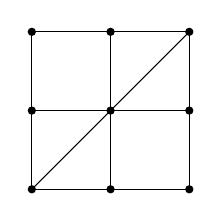
\begin{tikzpicture}
      \foreach \x in {0, 1, 2} {
        \foreach \y in {0, 1, 2} {
          \node [circ] at (\x, \y) {};
        }
      }
      \foreach \x in {0, 1, 2} {
        \draw (\x, 0) -- (\x, 2);
        \draw (0, \x) -- (2, \x);
      }
      \draw (0, 0) -- (2, 2);
    \end{tikzpicture}
  \end{center}
\end{eg}
It is easy to see that any line has exactly $[m]$ elements. We write $L^-$ and $L^+$ for the first and last point of the line, i.e.\ the points where the active coordinates are all $1$ and $m$ respectively. It is clear that any line $L$ is uniquely determined by $L^-$ and its active coordinates.

\begin{eg}
  In $[3]^3$, we have the line
  \[
    L = \{(1, 2, 1), (2, 2, 2), (3, 2, 3)\}.
  \]
  This is a line with $I = \{1, 3\}$ and $a_2 = 2$. The first and last points are $(1, 2, 1)$ and $(3, 2, 3)$.
\end{eg}

Then we have the following theorem:
\begin{thm}[Hales--Jewett theorem]\index{Hales--Jewett theorem}
  For all $m, k \in \N$, there exists $N = HJ(m, k)$ such that whenever $[m]^N$ is $k$-coloured, there exists a monochromatic line.
\end{thm}
Note that this theorem implies van der Waerden's theorem easily. The idea is to embed $[m]^N$ into $\N$ linearly, so that a monochromatic line in $[m]^N$ gives an arithmetic progression of length $m$. Explicitly, given a $k$-colouring $c: \N \to [k]$, we define $c': [m]^N \to [k]$ by
\[
  c'(x_1, x_2, \cdots, x_N) = c(x_1 + x_2 + \cdots + x_N).
\]
Now a monochromatic line gives us an arithmetic progression of length $m$. For example, if the line is
\[
  L = \{(1, 2, 1), (2, 2, 2), (3, 2, 3)\},
\]
then we get the monochromatic progression $4, 6, 8$ of length $3$. In general, the monochromatic AP defined has $d = |I|$.

The proof is essentially what we did for van der Waerden theorem. We are going to build a lot of almost-lines that point at the same vertex, and then no matter what colour the last vertex is, we are happy.

\begin{defi}[Focused lines]\index{focused lines}
  We say lines $L_1, \cdots, L_r$ are \emph{focused} at $f \in [m]^N$ if $L_i^+ = f$ for all $i = 1, \cdots, r$.
\end{defi}

\begin{defi}[Colour focused lines]\index{colour focused lines}\index{focused lines!colour}
  If $L_1, \cdots, L_r$ are focused lines, and $L_i \setminus \{L_i^+\}$ is monochromatic for each $i = 1, \cdots, r$ and all these colours are distinct, then we say $L_1, \cdots, L_r$ are \emph{colour focused} at $f$.
\end{defi}

\begin{proof}
  We proceed by induction on $m$. This is clearly trivial for $m = 1$, as a line only has a single point.

  Now suppose $m > 1$, and that $HJ(m - 1, k)$ exists for all $k \in \N$. As before, we will prove the following claim:
  \begin{claim}
    For each $1 \leq r \leq k$, there is an $n \in \N$ such that in any $k$-colouring of $[m]^n$, either
    \begin{enumerate}
      \item there exists a monochromatic line; or
      \item there exists $r$ colour-focused lines.
    \end{enumerate}
  \end{claim}
  Again, the result is immediate from the claim, as we just use it for $r = k$ and look at the colour of the focus.

  The prove this claim, we induct on $r$. If $r = 1$, then picking $n = HJ(m - 1, k)$ works, as a single colour-focused line of length $n$ is just a monochromatic line of length $n - 1$, and $[m - 1]^n \subseteq [m]^n$ naturally.

  Now suppose $r > 1$ and $n$ works for $r - 1$. Then we will show that $n + n'$ works, where
  \[
    n' = HJ(m - 1, k^{m^n}).
  \]
  Consider a colouring $c: [m]^{n + n'} \to [k]$, and we assume this has no monochromatic lines.

  We think of $[m]^{n + n'}$ as $[m]^n \times [m]^{n'}$. So for each point in $[m]^{n'}$, we have a whole cube $[m]^n$. Consider a $k^{m^n}$ colouring of $[m]^{n'}$ as follows --- given any $x \in [m]^{n'}$, we look at the subset of $[m]^{n + n'}$ containing the points with last $n'$ coordinates $x$. Then we define the new colouring of $[m]^{n'}$ to be the restriction of $c$ to this $[m]^n$, and there are $m^n$ possibilities.

  Now there exists a line $L$ such that $L \setminus L^+$ is monochromatic for the new colouring. This means for all $a \in [m]^n$ and for all $b, b' \in L\setminus L^+$, we have
  \[
    c(a, b) = c(a, b').
  \]
  Let $c''(a)$ denote this common colour for all $a \in [m]^n$. this is a $k$-colouring of $[m]^n$ with no monochromatic line (because $c$ doesn't have any). So by definition of $n$, there exists lines $L_1, L_2, \cdots, L_{r - 1}$ in $[m]^n$ which are colour-focused at some $f \in [m]^n$ for $c''$.

  In the proof of van der Waerden, we had a progression within each block, and also how we just between blocks. Here we have the same thing. We have the lines in $[m]^n$, and also the ``external'' line $L$.
  \begin{center}
    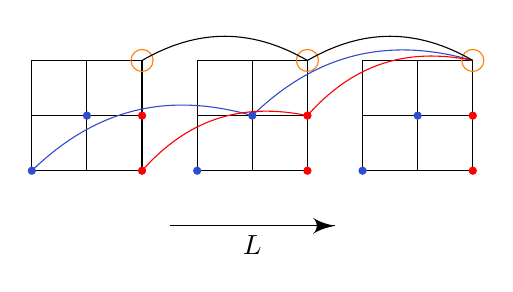
\begin{tikzpicture}[scale=0.7]
      \foreach \x in {0, 3, 6}{
        \begin{scope}[shift={(\x, 0)}]
          \draw [step=1] (0, 0) grid (2, 2);

          \node [circ, mblue] at (0, 0) {};
          \node [circ, mblue] at (1, 1) {};
          \node [circ, red] at (2, 0) {};
          \node [circ, red] at (2, 1) {};

          \draw [morange] (2, 2) circle [radius=0.2];
        \end{scope}
      }

      \draw [->] (2.5, -1) -- (5.5, -1) node [pos=0.5, below] {$L$} ;

      \draw [mblue] (0, 0) edge [bend left] (4, 1);
      \draw [mblue] (4, 1) edge [bend left] (8, 2);

      \draw [red] (2, 0) edge [bend left] (5, 1);
      \draw [red] (5, 1) edge [bend left] (8, 2);
      \draw (2, 2) edge [bend left] (5, 2);
      \draw (5, 2) edge [bend left] (8, 2);
    \end{tikzpicture}
  \end{center}
  Consider the line $L_1', L_2', \cdots, L_{r - 1}'$ in $[m]^{n + n'}$, where
  \[
    (L_i')^- = (L_i^-, L^-),
  \]
  and the active coordinate set is $I_i \cup I$, where $I$ is the active coordinate set of $L$.

  Also consider the line $F$ with $F^- = (f, L^-)$ and active coordinate set $I$.

  Then we see that $L_1', \cdots, L_{r - 1}', F$ are $r$ colour-focused lines with focus $(f, L^+)$.
\end{proof}

We can now prove our generalized van der Waerden.
\begin{thm}[Gallai]
  Whenever $\N^d$ is $k$-coloured, there exists a monochromatic (homothetic) copy of $S$ for each finite $S \subseteq \N^d$.
\end{thm}

\begin{proof}
  Let $S = \{S(1), S(2), \cdots, S(m)\} \subseteq \N^d$. Given a $k$-colouring $\N^d \to [k]$, we induce a $k$-colouring $c: [m]^N \to [k]$ by
  \[
    c'(x_1, \cdots, x_N) = c(S(x_1) + S(x_2) + \cdots + S(x_N)).
  \]
  By Hales-Jewett, for sufficiently large $N$, there exists a monochromatic line $L$ for $c'$, which gives us a monochromatic homothetic copy of $S$ in $\N^d$. For example, if the line is $(1\; 2\; 1)$, $(2\; 2\; 2)$ and $(3\; 2\; 3)$, then we know
  \[
    c(S(1) + S(2) + S(1)) = c(S(2) + S(2) + S(2)) = c(S(3) + S(2) + S(3)).
  \]
  So we have the monochromatic homothetic copy $\lambda S + \mu$ , where $\lambda = 2$ (the number of active coordinates), and $\mu = S(2)$.
\end{proof}

\subsubsection*{Largeness in Ramsey theory*}
In van der Waerden, we proved that for each $k, m$, there is some $n$ such that whenever we $k$-colour $[n]$, then there is a monochromatic AP of length $m$. How much of this is relies on the underlying set being $[n]$? Or is it just that if we finitely colour $[n]$, then one of the colours must contain a lot of numbers, and if we have a lot of numbers, then we are guaranteed to have a monochromatic AP?

Of course, by ``contains a lot of numbers'', we do not mean the actual number of numbers we have. It is certainly not true that for some $n$, whenever we $k$-colour any set of $n$ integers, we must have a monochromatic $m$-AP, because an arbitrary set of $n$ integers need not even contain an $m$-AP at all, let alone a monochromatic one. Thus, what we really mean is \emph{density}.
%
%We say $X \subseteq \N^{(2)}$ is \emph{large} if $X$ contains an infinite complete graph. Then Ramsey's theorem says if we finitely colour $\N$, then one of the colours gives a large subset.
%
%We say a $X \subseteq \N$ is large if $X$ contains an $m$ AP for all $m \in \N$. Again van der Waerden says if we finitely colour $\N$, then there is one colour that gives a large subset.
%
%But if we are lazy, then we might try to find such a large set simply by looking at the ``largest'' subset. So one natural question is as follows --- does a simpler ``counting'' notion of largeness imply Ramsey-theoretic structures?
%
%In $\N^{(2)}$ the answer is no, as there isn't much structure in $\N^{(2)}$, so we can only talk about whether things are infinite or not.
%
%However, in $\N$, we can talk about density.
\begin{defi}[Density]
 For $A \subseteq \N$, we let the \term{density} of $A$ as
 \[
   \bar{d}(A) = \limsup_{(b - a) \to \infty} \frac{A \cap [a, b]}{|b - a|}.
 \]
\end{defi}
Clearly, in any finite $k$-colouring of $\N$, there exists a colour class with positive density. Thus, we want to know if merely a positive density implies the existence of progressions. Remarkably, the answer is yes!

\begin{thm}[Szemer\'edi theorem]\index{Szemer\'edi theorem}
  Let $\delta > 0$ and $m \in \N$. Then there exists some $N = S(m, \delta) \in \N$ such that any subset $A \subseteq [N]$ with $|A| \geq \delta N$ contains an $m$-term arithmetic progression.
\end{thm}
The proof of this theorem is usually the subject of an entire lecture course, so we are not going to attempt to prove this. Even the particular case $m = 3$ is very hard.

This theorem has a lot of very nice Ramsey consequences. In the case of graph colourings, we asked ourselves what happens if we colour a graph with \emph{infinitely} many colours. Suppose we now have a colouring $c: \N \to \N$. Can we still find a monochromatic progression of length $m$? Of course not, because $c$ can be injective.

\begin{thm}
  For any $c: \N \to \N$, there exists a $m$-AP on which either
  \begin{enumerate}
    \item $c$ is constant; or
    \item $c$ is injective.
  \end{enumerate}
\end{thm}
It is also possible to prove this directly, but it is easy with Szemer\'edi.

\begin{proof}
  We set
  \[
    \delta = \frac{1}{m^2(m + 1)^2}.
  \]
  We let $N = S(m, \delta)$. We write
  \[
    [N] = A_1 \cup A_2 \cup \cdots \cup A_k,
  \]
  where the $A_i$'s are the colour-classes of $c|_{[N]}$. By choice of $N$, we are done if $|A_i| \geq \delta N$ for some $1 \leq i \leq k$. So suppose not.

  Let's try to count the number of arithmetic progressions in $[N]$. There are more than $N^2/(m + 1)^2$ of these, as we can take any $a, d \in [N/m + 1]$. We want to show that there is an AP that hits each $A_i$ at most once.

  So, fixing an $i$, how many AP's are there that hit $A_i$ at least twice? We need to pick two terms in $A_i$, and also decide which two terms in the progression they are in, e.g.\ they can be the first and second term, or the 5th and 17th term. So there are at most $m^2 |A_i|^2$ terms.

  So the number of AP's on which $c$ is injective is greater than
  \[
    \frac{N^2}{(m + 1)^2} - k |A_i|^2 m^2 \geq \frac{N^2}{(m + 1)^2} - \frac{1}{\delta} (\delta N)^2 m^2 = \frac{N^2}{(m + 1)^2} - \delta N^2 m^2 \geq 0.
  \]
  So we are done. Here the first inequality follows from the fact that $\sum |A_i| = [N]$ and each $|A_i| < \delta N$.
\end{proof}

Our next theorem will mix arithmetic and graph-theoretic properties. Consider a colouring $c: \N^{(2)} \to [2]$. As before, we say a set $X$ is monochromatic if $c|_{X^{(2)}}$ is constant. Now we want to try to find a monochromatic set with some arithmetic properties.

The first obvious question to ask is --- can we find a monochromatic 3-term arithmetic progression? The answer is no. For example, we can define $c(ij)$ to be the parity of largest power of $2$ dividing $j - i$, and then there is no monochromatic $3$-term arithmetic progression.

What if we make some concessions --- can we find a blue 10-AP, or if not, find an infinite red set? The answer is again no. This construction is slightly more involved. To construct a counterexample, we can make progressively larger red cliques, and take all other edges blue. If we double the size of the red cliques every time, it is not hard to check that there is no blue 4-AP, and no infinite red set.
\begin{center}
  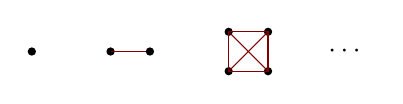
\begin{tikzpicture}
    \node [circ] at (0, 0) {};

    \node [circ] at (1, 0) {};
    \draw [mred] (1, 0) -- (1.5, 0);
    \node [circ] at (1.5, 0) {};

    \node [circ] at (2.5, 0.25) {};
    \node [circ] at (3, 0.25) {};
    \node [circ] at (2.5, -0.25) {};
    \node [circ] at (3, -0.25) {};

    \draw [mred] (2.5, 0.25) -- (2.5, -0.25) -- (3, -0.25) -- (3, 0.25) -- cycle;

    \draw [mred] (2.5, 0.25) -- (3, -0.25);
    \draw [mred] (2.5, -0.25) -- (3, 0.25);

    \node at (4, 0) {$\cdots$};
  \end{tikzpicture}
\end{center}
What if we further relax our condition, and only require an arbitrarily large red set?
\begin{thm}
  For any $c: \N^{(2)} \to \{\mathrm{red}, \mathrm{blue}\}$, either
  \begin{enumerate}
    \item There exists a blue $m$-AP for each $m \in \N$; or
    \item There exists arbitrarily large red sets.
  \end{enumerate}
\end{thm}

\begin{proof}
  Suppose we can't find a blue $m$-AP for some fixed $m$. We induct on $r$, and try to find a red set of size $r$.

  Say $A \subseteq \N$ is a progression of length $N$. Since $A$ has no blue $m$-term progression, so it must contain many red edges. Indeed, each $m$-AP in $A$ must contain a red edge. Also each edge specifies two points, and this can be extended to an $m$-term progression in at most $m^2$ ways. Since there are $N^2/(m + 1)^2$. So there are at least
  \[
    \frac{N^2}{m^2(m + 1)^2}
  \]
  red edges. With the benefit of hindsight, we set
  \[
    \delta = \frac{1}{2m^2(m + 1)^2}.
  \]
  The idea is that since we have lots of red edges, we can try to find a point with a lot of red edges connected to it, and we hope to find a progression in it.

  We say $X, Y \subseteq \N$ form an $(r, k)$-structure if
  \begin{enumerate}
    \item They are disjoint
    \item $X$ is red;
    \item $Y$ is an arithmetic progression;
    \item All $X\mdash Y$ edges are red;
    \item $|X| = r$ and $|Y| = k$.
  \end{enumerate} % insert a picture
  \begin{center}
    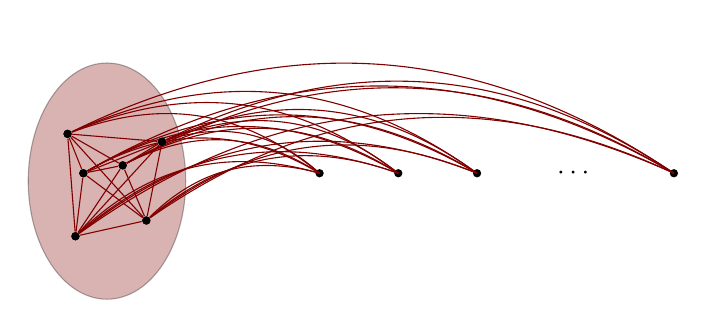
\begin{tikzpicture}
      \draw [fill=mred, opacity=0.3] (0.3, -0.1) ellipse (1 and 1.5);
      \node [circ] (1) at (0, 0) {};
      \node [circ] (2) at (1, 0.4) {};
      \node [circ] (3) at (0.5, 0.1) {};
      \node [circ] (4) at (-0.2, 0.5) {};
      \node [circ] (5) at (0.8, -0.6) {};
      \node [circ] (6) at (-0.1, -0.8) {};

      \draw [mred] (1) -- (2);
      \draw [mred] (1) -- (3);
      \draw [mred] (1) -- (4);
      \draw [mred] (1) -- (5);
      \draw [mred] (1) -- (6);
      \draw [mred] (2) -- (3);
      \draw [mred] (2) -- (4);
      \draw [mred] (2) -- (5);
      \draw [mred] (2) -- (6);
      \draw [mred] (3) -- (4);
      \draw [mred] (3) -- (5);
      \draw [mred] (3) -- (6);
      \draw [mred] (4) -- (5);
      \draw [mred] (4) -- (6);
      \draw [mred] (5) -- (6);

      \foreach \x in {3, 4, 5, 7.5} {
        \node [circ] at (\x, 0) {};
        \foreach \y in {1, 2, 3, 4, 5, 6} {
          \draw (\y) edge [bend left, mred] (\x, 0);
        }
      }
      \node at (6.25, 0) {$\cdots$};
      \node [circ] (1) at (0, 0) {};
      \node [circ] (2) at (1, 0.4) {};
      \node [circ] (3) at (0.5, 0.1) {};
      \node [circ] (4) at (-0.2, 0.5) {};
      \node [circ] (5) at (0.8, -0.6) {};
      \node [circ] (6) at (-0.1, -0.8) {};

    \end{tikzpicture}
  \end{center}
  We show by induction that there is an $(r, k)$-structure for each $r$ and $k$.

  A $(1, k)$ structure is just a vertex connected by red edges to a $k$-point structure. If we take $N = S(\delta, k)$, we know among the first $N$ natural numbers, there are at least $N^2/(m^2(m + 1)^2)$ red edges inside $[N]$. So in particular, some $v \in [N]$ has at least $\delta N$ red neighbours in $[N]$, and so we know $v$ is connected to some $k$-AP by red edges. That's the base case done.

  Now suppose we can find an $(r - 1, k')$-structure for all $k' \in \N$. We set
  \[
    k' = S\left(\frac{1}{2m^2(m + 1)^2}, k\right).
  \]
  We let $(X, Y)$ be an $(r - 1, k')$-structure. As before, we can find $v \in Y$ such that $v$ has $\delta|Y|$ red neighbours in $Y$. Then we can find a progression $Y'$ of length $k$ in the red neighbourhood of $v$, and we are done, as $(X \cup \{v\}, Y')$ is an $(r, k)$-structure, and an ``arithmetic progression'' within an arithmetic progression is still an arithmetic progression.
\end{proof}
Before we end this chapter, we make a quick remark. Everything we looked for in this chapter involved the additive structure of the naturals. What about the multiplicative structure? For example, given a finite colouring of $\N$, can we find a monochromatic geometric progression? The answer is trivially yes. We can look at $\{2^x: x \in \N\}$, and then multiplication inside this set just looks like addition in the naturals.

But what if we want to mix additive and multiplicative structures? For example, can we always find a monochromatic set of the form $\{x + y, xy\}$? Of course, there is the trivial answer $x = y = 2$, but is there any other? This question was answered positively in 2016! We will return to this at the end of the course.

\section{Partition Regularity}
In the previous chapter, the problems we studied were mostly ``linear'' in nature. We had some linear system, namely that encoding the fact that a sequence is an AP, and we wanted to know if it had a monochromatic solution. More generally, we can define the following:

\begin{defi}[Partition regularity]\index{partition regular}
  We say an $m \times n$ matrix $A$ over $\Q$ is \emph{partition regular} if whenever $\N$ is finitely coloured, there exists an $x \in \N^n$ such that $Ax = 0$ and $x$ is monochromatic, i.e.\ all coordinates of $x$ have the same colour.
\end{defi}
Recall that $\N$ does not include $0$.

There is no loss in generality by assuming $A$ in fact has entries in $\Z$, by scaling $A$, but sometimes it is (notationally) convenient to consider cases where the entries are rational.

The question of the chapter is the following --- when is a matrix partition regular? We begin by looking at some examples.
\begin{eg}[Schur's theorem]\index{Schur's theorem}
  \emph{Schur's theorem} says whenever $\N$ is finitely coloured, there exists a monochromatic set of the form $\{x, y, x + y\}$. In other words the matrix $\begin{pmatrix}1 & 1 & -1\end{pmatrix}$ is partition regular, since
  \[
    \begin{pmatrix}
      1 & 1 & -1
    \end{pmatrix}
    \begin{pmatrix}
      x\\y\\z
    \end{pmatrix} = 0 \Longleftrightarrow z = x + y.
  \]
\end{eg}

\begin{eg}
  How about $\begin{pmatrix}2 & 3 & -5\end{pmatrix}$. This is partition regular, because we can pick any $x$, and we have
  \[
    \begin{pmatrix}
      2 & 3 & -5
    \end{pmatrix}
    \begin{pmatrix}
      x\\x\\x
    \end{pmatrix} = 0.
  \]
  This is a trivial example.
\end{eg}

How about van der Waerden's theorem?
\begin{eg}
  Van der Waerden's theorem says there is a monochromatic $3$-AP $\{x_1, x_2, x_3\}$ whenever $\N$ is finitely-coloured. We know $x_1, x_2, x_3$ forms a $3$-AP iff
  \[
    x_3 - x_2 = x_2 - x_1,
  \]
  or equivalently
  \[
    x_3 + x_1 = 2 x_2.
  \]
  This implies that $\begin{pmatrix}1 & -2 & 1\end{pmatrix}$ is partition regular. But this is actually not a very interesting thing to say, because $x_1 = x_2 = x_3$ is always a solution to this equation. So this falls into the previous ``trivial'' case.

  On the second example sheet we saw a stronger version of van der Waerden. It says we can always find a monochromatic set of the form
  \[
    \{d, a, a + d, a + 2d, \cdots, a + md\}.
  \]
  By including this variable, we can write down the property of being a progression in a non-trivial format by
  \[
    \begin{pmatrix}
      1 & 1 & 0 & -1\\
      2 & 1 & -1 & 0
    \end{pmatrix}
    \begin{pmatrix}
      d \\ a \\ x_2 \\ x_3
    \end{pmatrix} = 0
  \]
  This obviously generalizes to an arbitrary $m$-AP, with matrix
  \[
    \begin{pmatrix}
      1 & 1 & -1 & 0 & 0 & \cdots & 0\\
      1 & 2 & 0 & -1 & 0 & \cdots & 0\\
      1 & 3 & 0 & 0 & -1 & \cdots & 0\\
      \vdots & \vdots & \vdots & \vdots & \vdots & \ddots & \vdots\\
      1 & m & 0 & 0 & 0 & \cdots & -1
    \end{pmatrix}.
  \]
\end{eg}
We've seen three examples of partition regular matrices. Of course, not every matrix is partition regular. The matrix $\begin{pmatrix}1 & 1\end{pmatrix}$ is not partition regular, for the silly reason that two positive things cannot add up to zero.

Let's now look at some non-trivial first matrix that is not partition regular.
\begin{eg}
  The matrix $\begin{pmatrix}2 & -1\end{pmatrix}$ is not partition regular, since we can put $c(x) = (-1)^n$, where $n$ is the maximum integer such that $2^n \mid x$. Then $\{x, 2x\}$ is never monochromatic.

  A similar argument shows that if $\lambda \in \Q$ is such that $\begin{pmatrix}\lambda, -1\end{pmatrix}$ is partition regular, then $\lambda = 1$.
\end{eg}
But if we write down a random matrix, say $\begin{pmatrix}2 & 3 & -6\end{pmatrix}$? The goal of this chapter is to find a complete characterization of matrices that are partition regular.

\begin{defi}[Columns property]\index{columns property}
  Let
  \[
    A =
    \begin{pmatrix}
      \uparrow & \uparrow & & \uparrow\\
      c^{(1)} & c^{(2)} & \cdots & c^{(n)}\\
      \downarrow & \downarrow & & \downarrow
    \end{pmatrix}.
  \]
  We say $A$ has the \emph{columns property} if there is a partition $[n] = B_1 \cup B_2 \cup \cdots \cup B_d$ such that
  \[
    \sum_{i \in B_s} c^{(i)} \in \spn\{c^{(i)} : c^{(i)} \in B_1 \cup \cdots \cup B_{s - 1}\}
  \]
  for $s = 1, \cdots, d$. In particular,
  \[
    \sum_{i \in B_1} c^{(i)} = 0
  \]
\end{defi}
What does this mean? Let's look at the matrices we've seen so far.
\begin{eg}
  $\begin{pmatrix}1 & 1 & -1\end{pmatrix}$ has the columns property by picking $B_1 = \{1, 3\}$ and $B_2 = \{2\}$.
\end{eg}

\begin{eg}
  $\begin{pmatrix}2 & 3 & -5\end{pmatrix}$ has the columns property by picking $B_1 = \{1, 2, 3\}$.
\end{eg}

\begin{eg}
  The matrix
  \[
    \begin{pmatrix}
      1 & 1 & -1 & 0 & 0 & \cdots & 0\\
      1 & 2 & 0 & -1 & 0 & \cdots & 0\\
      1 & 3 & 0 & 0 & -1 & \cdots & 0\\
      \vdots & \vdots & \vdots & \vdots & \vdots & \ddots & \vdots\\
      1 & m & 0 & 0 & 0 & \cdots & -1
    \end{pmatrix}
  \]
  has the column property. Indeed, we take $B_1 = \{1, 3, \cdots, m + 2\}$, and since $\{c^{(3)}, \cdots, c^{(m + 2)}\}$ spans all of $\R^m$, we know picking $B_2 = \{2\}$ works.
\end{eg}

\begin{eg}
  $\begin{pmatrix}\ell & -1\end{pmatrix}$ has the columns property iff $\ell = 1$. In particular, $\begin{pmatrix}1 & 1 \end{pmatrix}$ does not have a columns property.
\end{eg}

Given these examples, it is natural to conjecture the following:
\begin{thm}[Rado's theorem]\index{Rado's theorem}
  A matrix $A$ is partition regular iff it has the column property.
\end{thm}
This is a remarkable theorem! The property of being partition regular involves a lot of quantifiers, over infinitely many things, but the column property is entirely finite, and we can get a computer to check it for us easily.

Another remarkable property of this theorem is that neither direction is obvious! It turns out partition regularity implies the column property is (marginally) easier, because if we know something is partition regular, then we can try to cook up some interesting colourings and see what happens. The other direction is harder.

To get a feel of the result, we will first prove it in the case of a single equation. The columns property in particular becomes much simpler. It just means that there exists a non-empty subset of the non-zero $a_i$'s that sums up to zero.

\begin{thm}
  If $a_1,\cdots, a_n \in \Q \setminus \{0\}$, then $\begin{pmatrix} a_1 & \cdots & a_n \end{pmatrix}$ is partition regular iff there exists a non-empty $I \subseteq [n]$ such that
  \[
    \sum_{i \in I} a_i = 0.
  \]
\end{thm}

For a fixed prime $p$, we let $d(x)$ denote the last non-zero digit of $x$ in base $p$, i.e.\ if
\[
  x = d_n p^n + d_{n - 1}p^{n - 1} + \cdots + d_0,
\]
then
\[
  L(x) = \min\{i: d_i \not= 0\}
\]
and $d(x) = d_{L(x)}$. We now prove the easy direction of the theorem.

\begin{prop}
  If $a_2, \cdots, a_n \in \Q \setminus \{0\}$ and $\begin{pmatrix}a_1 & a_2 & \cdots & a_n\end{pmatrix}$ is partition regular, then
  \[
    \sum_{i \in I} a_i = 0
  \]
  for some non-empty $I$.
\end{prop}

\begin{proof}
  We wlog $a_i \in \Z$, by scaling. Fix a suitably large prime
  \[
    p > \sum_{i = 1}^n |a_i|,
  \]
  and consider the $(p - 1)$-colouring of $\N$ where $x$ is coloured $d(x)$. We find $x_1, \cdots, x_n$ such that
  \[
    \sum a_i x_i = 0.
  \]
  and $d(x_i) = d$ for some $d \in \{1, \cdots, p - 1\}$. We write out everything in base $p$, and let
  \[
    L = \min \{L(x_i): 1 \leq i \leq n\},
  \]
  and set
  \[
    I = \{i: L(x_i) = L\}.
  \]
  Then for all $i \in I$, we have
  \[
    x_i \equiv d \pmod {p^{L + 1}}.
  \]
  On the other hand, we are given that
  \[
    \sum a_i x_i = 0.
  \]
  Taking mod $p^{L + 1}$ gives us
  \[
    \sum_{i \in I} a_i d = 0 \pmod {p^{L + 1}}.
  \]
  Since $d$ is invertible, we know
  \[
    \sum_{i \in I} a_i = 0 \pmod {p^{L + 1}}.
  \]
  But by our choice of $p$, this implies that $\sum_{i \in I} a_i = 0$.
\end{proof}
Here we knew what prime $p$ to pick ahead. If we didn't, then we could consider \emph{all} primes $p$, and for each $p$ we find $I_p \subseteq [n]$ such that
\[
  \sum_{i \in I_p} a_i = 0 \pmod p.
\]
Then some $I_p$ has to occur infinitely often, and then we are done. Note that this is merely about the fact that if a fixed number is $0$ mod $n$ for arbitrarily large $n$, then it must be zero. This is not some deep local-global correspondence number theoretic fact.

It turns out this is essentially the only way we know for proving this theorem. One possible variation is to use the ``first non-zero digit'' to do the colouring, but this is harder.

Let's now try and do the other direction. Before we do that, we start by doing a warm up. Last time, we proved that if we had $\begin{pmatrix}1 & \lambda\end{pmatrix}$, then this is partition regular iff $\lambda = -1$. We now prove a three element version.

\begin{prop}
  The equation $\begin{pmatrix}1 & \lambda & -1\end{pmatrix}$ is partition regular for all $\lambda \in \Q$.
\end{prop}

\begin{proof}
  We may wlog $\lambda > 0$. If $\lambda = 0$, then this is trivial, and if $\lambda < 0$, then we can multiply the whole equation by $-1$.

  Say
  \[
    \lambda = \frac{r}{s}.
  \]
  The idea is to try to find solutions of this in long arithmetic progressions.

  Suppose $\N$ is $k$-coloured. We let
  \[
    \{a, a + d, \cdots, a + nd\}
  \]
  be a monochromatic AP, for $n$ sufficiently large.

  If $sd$ were the same colour as this AP, then we'd be done, as we can take
  \[
    x = a,\quad y = sd,\quad z = a + \frac{r}{s} sd.
  \]
  In fact, if any of $sd, 2sd, \cdots, \left\lfloor\frac{n}{r}\right\rfloor sd$ have the same colour as the AP, then we'd be done by taking
  \[
    x = a,\quad y = isd,\quad z = a + \frac{r}{s} isd = a + ird \leq a + nd.
  \]
  If this were not the case, then $\{sd, 2sd, \cdots, \left\lfloor\frac{n}{r}\right\rfloor sd\}$ is $(k - 1)$-coloured, and this is just a scaled up copy of $\N$. So we are done by induction on $k$.
\end{proof}

Note that when $\lambda = 1$, we have $\begin{pmatrix}1 & 1 & -1\end{pmatrix}$ is partition regular, and this may be proved by Ramsey's theorem. Can we prove this more general result by Ramsey's theorem as well? The answer is, we don't know.

It turns out this is not just a warm up, but the main ingredient of what we are going to do.

\begin{thm}
  If $a_1,\cdots, a_n \in \Q$, then $\begin{pmatrix} a_1 & \cdots & a_n \end{pmatrix}$ is partition regular iff there exists a non-empty $I \subseteq [n]$ such that
  \[
    \sum_{i \in I} a_i = 0.
  \]
\end{thm}

\begin{proof}
  One direction was done. To do the other direction, we recall that we had a really easy case of, say,
  \[
    \begin{pmatrix}
      2 & 3 & -5
    \end{pmatrix},
  \]
  because we can just make all the variables the same?

  In the general case, we can't quite do this, but we may try to solve this equation with the least number of variables possible. In fact, we shall find some monochromatic $x, y, z$, and then assign each of $x_1, \cdots, x_n$ to be one of $x, y, z$.

  We know
  \[
    \sum_{i \in I} a_i = 0.
  \]
  We now partition $I$ into two pieces. We fix $i_0 \in I$, and set
  \[
    x_i =
    \begin{cases}
      x & i = i_0\\
      y & i \in I \setminus \{i_0\}\\
      z & i \not\in I
    \end{cases}.
  \]
  We would be done if whenever we finitely colour $\N$, we can find monochromatic $x, y, z$ such that
  \[
    a_{i_0}x + \left(\sum_{i \in I \setminus \{i_0\}} a_i\right) z + \left(\sum_{i \not \in I} a_i\right) y = 0.
  \]
  But, since
  \[
    \sum_{i \in I} a_i = 0,
  \]
  this is equivalent to
  \[
    a_{i_0} x - a_{i_0} z + (\text{something}) y = 0.
  \]
  Since all these coefficients were non-zero, we can divide out by $a_{i_0}$, and we are done by the previous case.
\end{proof}

Note that our proof of the theorem shows that if an equation is partition regular for all last-digit base $p$ colourings, then it is partition regular for all colourings. This might sound like an easier thing to prove that the full-blown Rado's theorem, but it turns out the only proof we have for this implication is Rado's theorem.

We now prove the general case. We first do the easy direction, because it is largely the same as the single-equation case.

\begin{prop}
  If $A$ is an $m \times n$ matrix with rational entries which is partition regular, then $A$ has the columns property.
\end{prop}

\begin{proof}
  We again wlog all entries of $A$ are integers. Let the columns of $A$ be $c^{(1)}, \cdots, c^{(n)}$. Given a prime $p$, we consider the $(p - 1)$-colouring of $\N$, where $x$ is coloured $d(x)$, the last non-zero digit in the base $p$ expansion. Since $A$ is partition regular, we obtain a monochromatic solution.

  We then get a monochromatic $x_1, \cdots, x_n$ such that $Ax = 0$, i.e.
  \[
    \sum x_i c^{(i)} = 0.
  \]
  Any such solution with colour $d$ induces a partition of $[n] = B_1 \cup B_2 \cup \cdots \cup B_r$, where
  \begin{itemize}
    \item For all $i, j \in B_s$, we have $L(x_i) = L(x_j)$; and
    \item For all $s < t$ and $i \in B_s$, $j \in B_t$, the $L(x_i) < L(x_j)$.
  \end{itemize}
  Last time, with the benefit of hindsight, we were able to choose some large prime $p$ that made the argument work. So we use the trick we mentioned after the proof last time.

  Since there are finitely many possible partitions of $[n]$, we may assume that this particular partition is generated by infinitely many primes $p$. Call these primes $\mathcal{P}$. We introduce some notation. We say two vectors $u, v \in \Z^m$ satisfy $u \equiv v \pmod p$ if $u_i \equiv v_i \pmod p$ for all $i = 1, \cdots, m$.

  Now we know that
  \[
    \sum x_i c^{(i)} = 0.
  \]
  Looking at the first non-zero digit in the base $p$ expansion, we have
  \[
    \sum_{i \in B_1} d c^{(i)} \equiv 0 \pmod p.
  \]
  From this, we conclude that, by multiplying by $d^{-1}$
  \[
    \sum_{i \in B_1} c^{(i)} \equiv 0 \pmod p,
  \]
  for all $p \in \mathcal{P}$. So we deduce that
  \[
    \sum_{i \in B_1} c^{(i)} = 0.
  \]
  Similarly, for higher $s$, we find that for each base $p$ colouring, we have
  \[
    \sum_{i \in B_s} p^t d c^{(i)} + \sum_{i \in B_1 \cup \ldots \cup B_s} x_i c^{(i)} \equiv 0 \pmod {p^{t + 1}}
  \]
  for all $s \geq 2$, and some $t$ dependent on $s$ and $p$. Multiplying by $d^{-1}$, we find
  \[
    \sum_{i \in B_s} p^t c^{(i)} + \sum_{i \in B_1 \cup \ldots \cup B_{s - 1}} (d^{-1} x_i) c^{(i)} \equiv 0 \pmod {p^{t + 1}}.\tag{$*$}
  \]
  We claim that this implies
  \[
    \sum_{i \in \mathcal{B}_s} c^{(i)} \in \bra c^{(i)}: i \in B_1 \cup \cdots \cup B_{s - 1}\ket.
  \]
  This is not exactly immediate, because the values of $x_i$ in $(*)$ may change as we change our $p$. But it is still some easy linear algebra.

  Suppose this were not true. Since we are living in a Euclidean space, we have an inner product, and we can find some $v \in \Z^m$ such that
  \[
    \bra v, c^{(i)} \ket = 0\text{ for all }i \in B_1 \cup \cdots \cup B_{s - 1},
  \]
  and
  \[
    \left\bra v, \sum_{i \in B_s}c^{(i)}\right\ket \not= 0.
  \]
  But then, taking inner products with gives
  \[
    p^t \left\bra v, \sum_{i \in B_s} c^{(i)}\right\ket \equiv 0 \pmod {p^{t + 1}}.
  \]
  Equivalently, we have
  \[
    \left\bra v, \sum_{i \in B_s}c^{(i)}\right\ket \equiv 0 \pmod p,
  \]
  but this is a contradiction. So we showed that $A$ has the columns property with respect to the partition $[n] = B_1 \cup \cdots \cup B_r$.
\end{proof}

We now prove the hard direction. We want an analogous gadget to our $\begin{pmatrix}1 & \lambda & -1\end{pmatrix}$ we had for the single-equation case. The definition will seem rather mysterious, but it turns out to be what we want, and its purpose becomes more clear as we look at some examples.

\begin{defi}[$(m, p, c)$-set]\index{$(m, p, c)$-set}
  For $m, p, c \in \N$, a set $S \subseteq \N$ is an $(m, p, c)$-set with generators $x_1, \cdots, x_m$ if $S$ has the form
  \[
    S = \left\{ \sum_{i = 0}^m \lambda_i x_i : \begin{array}{c}\lambda_i = 0 \text{ for all }i < j\\ \lambda_j = c\\ \lambda_i \in [-p, p]\end{array}\right\}.
  \]
  In other words, we have
  \[
    S = \bigcup_{j = 1}^m \{c x_j + \lambda_{j + 1} x_{j + 1} + \cdots + \lambda_m x_m : \lambda_i \in [-p, p]\}.
  \]
  For each $j$, the set $\{c x_j + \lambda_{j + 1} x_{j + 1} + \cdots + \lambda_m x_m: \lambda_i \in [-p, p]\}$ is called a \emph{row} of $S$.
\end{defi}

\begin{eg}
  What does a $(2, p, 1)$ set look like? It has the form
  \[
    \{x_1 - p x_2, x_1 - (p - 1) x_2, \cdots, x_1 + p x_2\} \cup \{x_2\}.
  \]
  In other words, this is just an arithmetic progression with its common difference.
\end{eg}

\begin{eg}
  A $(2, p, 3)$-set has the form
  \[
    \{3x_1 - p x_2, \cdots, 3 x_1, \cdots, 3 x_1 = p x_2\} \cup \{3 x_2\}.
  \]
\end{eg}
The idea of an $(m, p, c)$ set is that we ``iterate'' this process many times, and so an $(m, p, c)$-set is an ``iterated AP's and various patterns of their common differences''.

Our proof strategy is to show that that whenever we finitely-colour $\N$, we can always find an $(m, p, c)$-set, and given any matrix $A$ with the columns property and any $(m, p, c)$-set (for suitable $m$, $p$, $c$), there will always be a solution in there.

\begin{prop}
  Let $m, p, c \in \N$. Then whenever $\N$ is finitely coloured, there exists a monochromatic $(m, p, c)$-set.
\end{prop}

\begin{proof}
  It suffices to find an $(m, p, c)$-set all of whose rows are monochromatic, since when $\N$ is $k$-coloured, and $(m', p, c)$-set with $m' = mk + 1$ has $m$ monochromatic rows of the same colour by pigeonhole, and these rows contain a monochromatic $(m, p, c)$-set, by restricting to the elements where a lot of the $\lambda_i$ are zero. In this proof, whenever we say $(m, p, c)$-set, we mean one all of whose rows are monochromatic.

  We will prove this by induction. We have a $k$-colouring of $[n]$, where $n$ is very very very large. This contains a $k$-colouring of
  \[
    B = \left\{c, 2c, \cdots, \left\lfloor \frac{n}{c}\right\rfloor c\right\}.
  \]
  Since $c$ is fixed, we can pick this so that $\frac{n}{c}$ is large. By van der Waerden, we find some set monochromatic
  \[
    A = \{c x_1 - Nd, cx_1 - (N - 1)d, \cdots, cx_1 + Nd \} \subseteq B,
  \]
  with $N$ very very large. Since each element is a multiple of $c$ by assumption, we know that $c \mid d$. By induction, we may find an $(m - 1, p, c)$-set in the set $\{d, 2d, \cdots, Md\}$, where $M$ is large. We are now done by the $(m, p, c)$ set on generators $x_1, \cdots, x_n$, provided
  \[
    c x_1 + \sum_{i = 2}^m \lambda_i x_i \in A
  \]
  for all $\lambda_i \in [-p, p]$, which is easily seen to be the case, provided $N \geq (m - 1) pM$.
\end{proof}
Note that the argument itself is quite similar to that in the $\begin{pmatrix}1 & \lambda & -1\end{pmatrix}$ case.

Recall that Schur's theorem said that whenever we finitely-colour $\N$, we can find a monochromatic $\{x, y , x + y\}$. More generally, for $x_1, x_2, \cdots, x_m \in \N$, we let
\[
  FS(x_1, \cdots, x_m) = \left\{\sum_{i \in I} x_i : I \subseteq [n], I \not= \emptyset\right\}.
\]
The existence of a monochromatic $(m, 1, 1)$-sets gives us
\begin{cor}[Finite sum theorem]\index{Finite sum theorem}
  For every fixed $m$, whenever we finitely-colour $\N$, there exists $x_1, \cdots, x_m$ such that $FS(x_1, \cdots, x_m)$ is monochromatic.
\end{cor}
This is since an $(m, 1, 1)$-set contains more things than $FS(x_1, \cdots, x_m)$. This was discovered independently by a bunch of different people, including Folkman, Rado and Sanders.

Similarly, if we let
\[
  FP(x_1, \cdots, x_m) = \left\{\prod_{i \in I} x_i : I \subseteq [n], I \not= \emptyset\right\},
\]
then we can find these as well. For example, we can restrict attention to $\{2^n: n \in \N\}$, and use the finite sum theorem. This is the same idea as we had when we used van der Waerden to find geometric progressions.

But what if we want both? Can we have $FS(x_1,\cdots, x_m) \cup FP(x_1, \cdots, x_m)$ in the same colour class? The answer is actually not known! Even the case when $m = 2$, i.e.\ finding a monochromatic set of the form $\{x, y, x + y, xy\}$ is open. Until mid 2016, we did not know if we can find $\{x + y, xy\}$ monochromatic ($x, y > 2$).

To finish he proof of Rado's theorem, we need the following proposition:
\begin{prop}
  If $A$ is a rational matrix with the columns property, then there is some $m, p, c \in \N$ such that $Ax = 0$ has a solution inside any $(m, p, c)$ set, i.e.\ all entries of the solution lie in the $(m, p, c)$ set.
\end{prop}
In the case of a single equation, we reduced the general problem to the case of 3 variables only. Here we are going to do something similar --- we will use the columns property to reduce the solution to something much smaller.

\begin{proof}
  We again write
  \[
    A =
    \begin{pmatrix}
      \uparrow & \uparrow & & \uparrow\\
      c^{(1)} & c^{(2)} & \cdots & c^{(n)}\\
      \downarrow & \downarrow & & \downarrow
    \end{pmatrix}.
  \]
  Re-ordering the columns of $A$ if necessary, we assume that we have
  \[
    [n] = B_1 \cup \cdots \cup B_r
  \]
  such that $\max(B_s) < \min(B_{s + 1})$ for all $s$, and we have
  \[
    \sum_{i \in B_s} c^{(i)} = \sum_{i \in B_1 \cup \ldots \cup B_{s - 1}} q_{is}c^{(i)}
  \]
  for some $q_{is} \in \Q$. These $q_{is}$ only depend on the matrix. In other words, we have
  \[
    \sum d_{is} c^{(i)} = 0,
  \]
  where
  \[
    d_{is} =
    \begin{cases}
      -q_{is} & i \in B_1 \cup \cdots B_{s - 1}\\
      1 & i \in B_s\\
      0 & \text{otherwise}
    \end{cases}
  \]
  For a fixed $s$, if we scan these coefficients starting from $i = n$ and then keep decreasing $i$, then the first non-zero coefficient we see is $1$, which is good, because it looks like what we see in an $(m, p, c)$ set.

  Now we try to write down a general solution with $r$ many free variables. Given $x_1, \cdots, x_r \in \N^r$, we look at
  \[
    y_i = \sum_{s = 1}^r d_{is}x_s.
  \]
  It is easy to check that $Ay = 0$ since
  \[
    \sum y_i c^{(i)} = \sum_i \sum_s d_{is} x_s c^{(i)} = \sum_s x_s \sum_i d_{is} c^{(i)} = 0.
  \]
  Now take $m = r$, and pick $c$ large enough such that $c d_{is} \in \Z$ for all $i, s$, and finally, $p = \max \{c d_{is}: i, s \in \Q\}$.

  Thus, if we consider the $(m, p, c)$-set on generators $(x_m, \cdots, x_1)$ and $y_i$ as defined above, then we have $Ay = 0$ and hence $A(cy) = 0$. Since $cy$ is integral, and lies in the $(m, p, c)$ set, we are done!
\end{proof}

We have thus proved Rado's theorem.
\begin{thm}[Rado's theorem]\index{Rado's theorem}
  A matrix $A$ is partition regular iff it has the column property.
\end{thm}
So we have a complete characterization of all partition regular matrices.

Note that Rado's theorem reduces Schur's theorem, van der Waerden's theorem, finite sums theorem etc. to just checking if certain matrices have the columns property, which are rather straightforward computations.

More interestingly, we can prove some less obvious ``theoretical'' results.

\begin{cor}[Consistency theorem]\index{consistency theorem}
  If $A$, $B$ are partition regular in independent variables, then
  \[
    \begin{pmatrix}
      A & 0\\
      0 & B
    \end{pmatrix}
  \]
  is partition regular. In other words, we can solve $Ax = 0$ and $By = 0$ simultaneously in the same colour class.
\end{cor}

\begin{proof}
  The matrix
  \[
    \begin{pmatrix}
      A & 0\\
      0 & B
    \end{pmatrix}
   \]
   has the columns property if $A$ and $B$ do.
\end{proof}
In fact, much much more is true.

\begin{cor}
  Whenever $\N$ is finitely-coloured, one colour class contains solutions to \emph{all} partition regular systems!
\end{cor}

\begin{proof}
  Suppose not. Then we have $\N = D_1 \cup \cdots \cup D_k$ such that for each $D_i$, there is some partition regular matrix $A_i$ such that we cannot solve $A_i x = 0$ inside $D_i$. But this contradicts the fact that $\diag(A_1, A_2, \cdots, A_k)$ is partition regular (by applying consistency theorem many times).
\end{proof}

Where did this whole idea of the $(m, p, c)$-sets come from? The original proof by Rado didn't use $(m, p, c)$-sets, and this idea only appeared only a while later, when we tried to prove a more general result.

In general, we call a set $D \subseteq \N$ \emph{partition regular} if we can solve any partition regular system in $D$. Then we know that $\N, 2\N$ are partition regular sets, but $2\N + 1$ is not (because we can't solve $x + y = z$, say). Then what Rado's theorem says is that whenever we finitely partition $\N$, then one piece of $\N$ is partition regular.

In the 1930's, Rado conjectured that there is nothing special about $\N$ to begin with --- whenever we break up a partition regular set, then one of the pieces is partition regular. This conjecture was proved by Deuber in the 1970s who introduced the idea of the $(m, p, c)$-set.

It is not hard to check that $D$ is partition regular iff $D$ contains an $(m, p, c)$ set of each size. Then Deuber's proof involves showing that for all $m, p, c, k \in \N$, there exists $n, q, d \in \N $ such that any $k$-colouring of an $(n, q, d)$-set contains a monochromatic $(m, p, c)$ set. The proof is quite similar to how we found $(m, p, c)$-sets in the naturals, but instead of using van der Waerden theorem, we need the Hales--Jewett theorem.

\separator

We end by mentioning an open problem in this area. Suppose $A$ is an $m \times n $ matrix $A$ that is not partition regular. That is, there is some $k$-colouring of $\N$ with no solution to $Ax = 0$ in a colour class. Can we find some bound $f(m, n)$, such that every such $A$ has a ``bad'' colouring with $k < f(m, n)$? This is an open problem, first conjectured by Rado, and we think the answer is yes.

What do we actually know about this problem? The answer is trivially yes for $f(1, 2)$, as there aren't many matrices of size $1 \times 2$, up to rescaling. It is a non-trivial theorem that $f(1, 3)$ exists, and in fact $f(1, 3) \leq 24$. We don't know anything more than that.

\section{Topological Dynamics in Ramsey Theory}
Recall the finite sum theorem --- for any fixed $k$, whenever $\N$ is finitely coloured, we can find $x_1, \cdots, x_k$ such that $FS(x_1, x_2, \cdots, x_k)$ is monochromatic. One natural generalization is to ask the following question --- can we find an infinite set $A$ such that
\[
  FS(A) = \left\{\sum_{x \in B} x : B \subseteq A\text{ finite non-empty}\right\}
\]
is monochromatic? The first thought upon hearing this question is probably either ``this is so strong that there is no way it can be true'', or ``we can deduce it easily, perhaps via some compactness argument, from the finite sum theorem''.

Both of these thoughts are wrong. It is true that it is always possible to find these $x_1, x_2, \cdots$, but the proof is hard. This is \emph{Hindman's theorem}.

The way we are going to approach this is via \emph{topological dynamics}, which is the title of this chapter. The idea is we construct a metric space (and in particular a \emph{dynamical system}) out of the Ramsey-theoretic problem we are interested in, and then convert the Ramsey-theoretic problem into a question about topological properties of the space we are constructed.

In the case of Hindman's theorem, it turns out the ``topological'' form is a general topological fact, which we can prove for a general dynamical system. What is the advantage of this approach? When we construct the dynamical system we are interested in, what we get is highly ``non-geometric''. It would be very difficult to think of it as an actual ``space''. It is just something that happens to satisfy the definition of a metric space. However, when we prove the general topological facts, we will think of our metric space as a genuine space like $\R^n$, and this makes it much easier to visualize what is going on in the proofs.

A less obvious benefit of this approach is that we will apply Tychonoff's theorem many times, and also use the fact that the possibly infinite intersection of nested compact sets is open. If we don't formulate our problem in topological terms, then we might find ourselves re-proving these repeatedly, which further complicates the proof.

We now begin our journey.

\begin{defi}[Dynamical system]\index{dynamical system}
  A \emph{dynamical system} is a pair $(X, T)$ where $X$ is the compact metric space and $T$ is a homeomorphism on $X$.
\end{defi}

\begin{eg}
  $(T = \R/Z, T_\alpha(x) = x + \alpha)$ for $\alpha \in \R$ is a dynamical system.
\end{eg}
In this course, this is not the dynamical system we are interested in. In fact, we are only ever going to be interested in one dynamical system.

We fix number of colours $k \in \N$. Instead of looking at a particular colouring, we consider the space of all $k$-colourings. We let
\[
  \mathcal{C} = \{c: \Z \to [k]\} \cong [k]^{\Z}.
\]
We endow this with the product topology. Since $[k]$ has the discrete topology, our basic open sets have the form
\[
  U = \{c: \Z \to [k] : c(i_1) = c_1, \cdots, c(i_s) = c_s\}
\]
for some $i_1, \cdots, i_s \in \Z$ and $c_1, \cdots, c_s \in [k]$.

Since $[k]$ is trivially compact, by Tychonoff's theorem, we know that $\mathcal{C}$ is compact. But we don't really need Tychonoff, since we know that $\mathcal{C}$ is metrizable, with metric
\[
  \rho(c_1, c_2) = \frac{1}{n + 1},
\]
where $n$ is the largest integer for which $c_1$ and $c_2$ agree on $[-n, n]$. This metric is easily seen to give rise to the same topology, and by hand, we can see this is sequentially compact.

We now have to define the operation on $\mathcal{C}$ we are interested in.
\begin{defi}[Left shift]\index{left shift}\index{$\mathcal{L}$}
  The \emph{left shift} operator $\mathcal{L}: \mathcal{C} \to \mathcal{C}$ is defined by
  \[
    (\mathcal{L}c)(i) = c(i + 1).
  \]
\end{defi}
\begin{center}
  \begin{tikzpicture}
    \foreach \x in {-2,-1,1,2} {
      \node [mblue, circ] at (\x, 0) {};
    }
    \node [mred, circ] at (0, 0) {};
    \begin{scope}[shift={(7, 0)}]
      \foreach \x in {-2,0,1,2} {
        \node [mblue, circ] at (\x, 0) {};
      }
      \node [mred, circ] at (-1, 0) {};
    \end{scope}
    \draw [->] (3, 0) -- (4, 0);
  \end{tikzpicture}
\end{center}
We observe that this map is invertible, with inverse given by the right shift. This is one good reason to work over $\Z$ instead of $\N$. Moreover, we see that $\mathcal{L}$ is nice and uniformly continuous, since if
\[
  \rho(c_1, c_2) \leq \frac{1}{n + 1},
\]
then
\[
  \rho(\mathcal{L} c_1, \mathcal{L} c_2) \leq \frac{1}{n}.
\]
Similarly, $\mathcal{L}^{-1}$ is uniformly continuous. So it follows that $(\mathcal{C}, \mathcal{L})$ is a dynamical system.

Instead of proving Hindman's theorem directly, we begin by re-proving van der Waerden's theorem using this approach, to understand better how it works.

\begin{thm}[Topological van der Waerden]\index{topological van der Waerden theorem}\index{van der Waerden theorem!topological}
  Let $(X, T)$ be a dynamical system. Then there exists an $\varepsilon > 0$ such that whenever $r \in\N$, then we can find $x \in X$ and $n \in \N$ such that $\rho(x, T^{in} x) < \varepsilon$ for all $i = 1, \cdots, r$.
\end{thm}
In words, this says if we flow around $X$ under $T$, then eventually some point must go back near to itself, and must do that as many times as we wish to, in regular intervals.

To justify calling this the topological van der Waerden theorem, we should be able to easily deduce van der Waerden's theorem from this. It is not difficult to imagine this is vaguely related to van der Waerden in some sense, but it is not obvious how we can actually do the deduction. After all, topological van der Waerden theorem talks about the whole space of all colourings, and we do not get to control what $x$ we get back from it. What we want is to start with a single colouring $c$ and try to say something about this particular $c$.

Now of course, we cannot restrict to the sub-system consisting only of $c$ itself, because, apart from it being really silly, the function $\mathcal{L}$ does not restrict to a map $\{c\} \to \{c\}$. We might think of considering the set of all translates of $c$. While this is indeed closed under $\mathcal{L}$, this is not a dynamical system, since it is not compact! The solution is to take the closure of that.

\begin{defi}[Orbital closure]\index{orbital closure}
  Let $(X, T)$ be a dynamical system, and $x \in X$. The \emph{orbital closure} $\bar{x}$ of $x$ is the set $\cl \{T^s x: s \in \Z\}$.
\end{defi}
Observe that $\bar{x}$ is a closed subset of a compact space, hence compact.

\begin{prop}
  $(\bar{X}, T)$ is a dynamical system.
\end{prop}

\begin{proof}
  It suffices to show that $\bar{x}$ is closed under $T$. If $y \in \bar{x}$, then we have some $s_i$ such that $T^{s_i}x \to y$. Since $T$ is continuous, we know $T^{s_i + 1}x \to T y$. So $T y \in \bar{x}$. Similarly, $T^{-1}\bar{x} = \bar{x}$.
\end{proof}

Once we notice that we can produce such a dynamical system from our favorite point, it is straightforward to prove van der Waerden.
\begin{cor}[van der Waerden theorem]\index{van der Waerden theorem}
  Let $r, k \in \N$. Then whenever $\Z$ is $k$-coloured, then there is a monochromatic arithmetic progression of length $r$.
\end{cor}

\begin{proof}
  Let $c: \Z \to [k]$. Consider $(\bar{c}, \mathcal{L})$. By topological van der Waerden, we can find $x \in \bar{c}$ and $n \in \N$ such that $\rho(x, \mathcal{L}^{in} x) < 1$ for all $i = 1, \cdots, r$. In particular, we know that $x$ and $\mathcal{L}^{in} x$ agree at $0$. So we know that
  \[
    x(0) = \mathcal{L}^{in} x(0) = x(in)
  \]
  for all $i = 0, \cdots, r$.

  We are not quite done, because we just know that $x \in \bar{c}$, and not that $x = \mathcal{L}^k x$ for some $k$.

  But this is not bad. Since $x \in \bar{c}$, we can find some $s \in \Z$ such that
  \[
    \rho(T^s c, x) \leq \frac{1}{rn + 1}.
  \]
  This means $x$ and $T^s c$ agree on the first $rn + 1$ elements. So we know
  \[
    c(s) = c(s + n) = \cdots = c(s + rn).\qedhere
  \]
\end{proof}
Since we will be looking at these $\bar{c}$ a lot, it is convenient to figure out what this $\bar{c}$ actually looks like. It turns out there is a reasonably good characterization of these orbital closures.

Let's look at some specific examples. Consider $c$ given by
\begin{center}
  
\begin{tikzpicture}[scale=0.6]
    \foreach \x in {-1, 1} {
      \node [mblue, circ] at (\x, 0) {};
    }
    \foreach \x in {-2,0,2} {
      \node [mred, circ] at (\x, 0) {};
    }
  \end{tikzpicture}
\end{center}
Then the orbital closure has just two points, $c$ and $\mathcal{L} c$.

What if we instead had the following?
\begin{center}
  
\begin{tikzpicture}[scale=0.6]
    \foreach \x in {-3,-2,-1} {
      \node [mblue, circ] at (\x, 0) {};
    }
    \foreach \x in {0,1,2,3} {
      \node [mred, circ] at (\x, 0) {};
    }
  \end{tikzpicture}
\end{center}
Then $\bar{c}$ contains all translates of these, but also
\begin{center}
  
\begin{tikzpicture}[scale=0.6]
    \foreach \x in {-3,-2,-1,0,1,2,3} {
      \node [mblue, circ] at (\x, 0) {};
    }
  \end{tikzpicture}
  ,
  \quad
  
\begin{tikzpicture}[scale=0.6]
    \foreach \x in {-3,-2,-1,0,1,2,3} {
      \node [mred, circ] at (\x, 0) {};
    }
  \end{tikzpicture}
\end{center}
We define the following:
\begin{defi}[$\Seq$]\index{$\Seq$}
  Let $c: \Z \to [k]$. We define
  \[
    \Seq (c) = \{(c(i), \cdots, c(i + r)): i \in \Z, r \in \N\}.
  \]
\end{defi}
It turns out these sequences tell us everything we want to know about orbital closures.

\begin{prop}
  We have $c' \in \bar{c}$ iff $\Seq(c') \subseteq \Seq(c)$.
\end{prop}
The proof is just following the definition and checking everything works.
\begin{proof}
  We first prove $\Rightarrow$. Suppose $c' \in \bar{c}$. Let $(c'(i) , \cdots, c'(i + r - 1)) \in \Seq(c)$. Then we have $s \in \Z$ such that
  \[
    \rho(c', \mathcal{L}^s c) < \frac{1}{1 + \max(|i|, |i + s - 1|)},
  \]
  which implies
  \[
    (c(s + i), \cdots, c(s + i + r - 1)) = (c'(i), \cdots, c'(i + s - 1)).
  \]
  So we are done.

  For $\Leftarrow$, if $\Seq(c') \subseteq \Seq (c)$, then for all $n \in \N$, there exists $s_n \in \Z$ such that
  \[
    (c'(-n), \cdots, c'(n)) = (c(s_n - n), \cdots, c(s_n + n)).
  \]
  Then we have
  \[
    \mathcal{L}^{s_i} c \to c'.
  \]
  So we have $c' \in \bar{c}$.
\end{proof}

We now return to talking about topological dynamics. We saw that in our last example, the orbital closure of $c$ has three ``kinds'' of things --- translates of $c$, and the all-red and all-blue ones. The all-red and all-blue ones are different, because they seem to have ``lost'' the information of $c$. In fact, the orbital closure of each of them is just that colouring itself. This is a \emph{strict} subset of $\bar{c}$. These are phenomena we don't want.
\begin{defi}[Minimal dynamical system]\index{minimal dynamical system}\index{dynamical system!minimal}
  We say $(X, T)$ is \emph{minimal} if $\bar{x} = X$ for all $x \in X$. We say $x \in X$ is \emph{minimal} if $(\bar{x}, T)$ is a minimal dynamical system.
\end{defi}

\begin{prop}
  Every dynamical system $(X, T)$ has a minimal point.
\end{prop}
Thus, most of the time, when we want to prove something about dynamical systems, we can just pass to a minimal subsystem, and work with it.

\begin{proof}
  Let $\mathcal{U} = \{\bar{x}: x \in X\}$. Thus is a family of closed sets, ordered by inclusion. We want to apply Zorn's lemma to obtain a minimal element. Consider a chain $S$ in $\mathcal{U}$. If
  \[
    \bar{x}_1 \supseteq \bar{x}_2 \supseteq \cdots \supseteq \bar{x}_n,
  \]
  then their intersection is $\bar{x}_n$, which is in particular non-empty. So any finite collection in $S$ has non-empty intersection. Since $X$ is compact, we know
  \[
    \bigcap_{\bar{x} \in S} \bar{x} \not= \emptyset.
  \]
  We pick
  \[
    z \in \bigcap_{\bar{x} \in S} \bar{x} \not= \emptyset.
  \]
  Then we know that
  \[
    \bar{z} \subseteq \bar{x}
  \]
  for all $\bar{x} \in S$. So we know
  \[
    \bar{z} \subseteq \bigcap_{\bar{x} \in S} \bar{x} \not= \emptyset.
  \]
  So by Zorn's lemma, we can find a minimal element (in both senses).
\end{proof}

\begin{eg}
  Consider $c$ given by
  \begin{center}
    
\begin{tikzpicture}[scale=0.6]
      \foreach \x in {-3,-2,-1} {
        \node [mblue, circ] at (\x, 0) {};
      }
      \foreach \x in {0,1,2,3} {
        \node [mred, circ] at (\x, 0) {};
      }
    \end{tikzpicture}
  \end{center}
  Then we saw that $\bar{c}$ contains all translates of these, and also
  \begin{center}
    
\begin{tikzpicture}[scale=0.6]
      \foreach \x in {-3,-2,-1,0,1,2,3} {
        \node [mblue, circ] at (\x, 0) {};
      }
    \end{tikzpicture}
    ,
    \quad
    
\begin{tikzpicture}[scale=0.6]
      \foreach \x in {-3,-2,-1,0,1,2,3} {
        \node [mred, circ] at (\x, 0) {};
      }
    \end{tikzpicture}
  \end{center}
  Then this system is not minimal, since the orbital closure of the all-red one is a strict subsystem of $\bar{c}$.
\end{eg}

We are now going to derive some nice properties of minimal systems.
\begin{lemma}
  If $(X, T)$ is a minimal system, then for all $\varepsilon > 0$, there is some $m \in \N$ such that for all $x, y \in X$, we have
  \[
    \min_{|s| \leq m} \rho(T^s x, y) < \varepsilon.
  \]
\end{lemma}

\begin{proof}
  Suppose not. Then there exists $\varepsilon > 0$ and points $x_i, y_i \in X$ such that
  \[
    \min_{|s| \leq i} \rho(T^s x_i, y_i) \geq \varepsilon.
  \]
  By compactness, we may pass to subsequences, and assume $x_i \to x$ and $y_i \to y$. By continuity, it follows that
  \[
    \rho(T^s x, y) \geq \varepsilon
  \]
  for all $s \in \Z$. This is a contradiction, since $\bar{x} = X$ by minimality.
\end{proof}
We now want to prove topological van der Waerden.
\begin{thm}[Topological van der Waerden]\index{topological van der Waerden theorem}\index{van der Waerden theorem!topological}
  Let $(X, T)$ be a dynamical system. Then there exists an $\varepsilon > 0$ such that whenever $r \in\N$, then we can find $x \in X$ and $n \in \N$ such that $\rho(x, T^{in} x) < \varepsilon$ for all $i = 1, \cdots, r$.
\end{thm} % this needs some pictures

\begin{proof}
  Without loss of generality, we may assume $(X, T)$ is a minimal system. We induct on $r$. If $r = 1$, we can just choose $y \in X$, and consider $T y, T^2 y, \cdots$. Then note that by compactness, we have $s_1, s_2 \in \N$ such that
  \[
    \rho(T^{s_1} y,T^{s_2} y) < \varepsilon,
  \]
  and then take $x = T^{s_1} y$ and $n = s_2 - s_1$.

  Now suppose the result is true for $r > 1$, and that we have the result for all $\varepsilon > 0$ and $r - 1$.
  \begin{claim}
    For all $\varepsilon > 0$, there is some point $y \in X$ such that there is an $x \in X$ and $n \in \N$ such that
    \[
      \rho(t^{in} x, y) < \varepsilon
    \]
    for all $1 \leq i \leq r$.
  \end{claim}
  Note that this is a different statement from the theorem, because we are not starting at $x$. In fact, this is a triviality. Indeed, let $(x_0, n)$ be as guaranteed by the hypothesis. That is, $\rho(x_0, T^{in}x_0) < \varepsilon$ for all $1 \leq i \leq r$. Then pick $y = x_0$ and $x = T^{-n}x_0$.

  The next goal is to show that there is nothing special about this $y$.
  \begin{claim}
    For all $\varepsilon > 0$ and for all $z \in X$, there exists $x_z \in X$ and $n \in \N$ for which $\rho(T^{in} x_z, z) < \varepsilon$.
  \end{claim}
  The idea is just to shift the picture so that $y$ gets close to $z$, and see where we send $x$ to. We will use continuity to make sure we don't get too far away.

  We choose $m$ as in the previous lemma for $\frac{\varepsilon}{2}$. Since $T^{-m}, T^{-m + 1}, \cdots, T^m$ are all uniformly continuous, we can choose $\varepsilon'$ such that $\rho(a, b) < \varepsilon'$ implies $\rho(T^s a, T^s b) < \frac{\varepsilon}{2}$ for all $|s| \leq m$.

  Given $z \in X$, we obtain $x$ and $y$ by applying our first claim to $\varepsilon'$. Then we can find $s \in \Z$ with $|s| \leq m$ such that $\rho(T^s y, z) < \frac{\varepsilon}{2}$. Consider $x_z = T^s x$. Then
  \begin{align*}
    \rho(T^{in} x_z, z) &\leq \rho(T^{in} x_z, T^s y) + \rho(T^s y, z) \\
    &\leq \rho(T^s(T^{in}x), T^s y) + \frac{\varepsilon}{2}\\
    &\leq \frac{\varepsilon}{2} + \frac{\varepsilon}{2}\\
    &= \varepsilon
  \end{align*}

  \begin{claim}
    For all $\varepsilon > 0$ and $z \in X$, there exists $x \in X$, $n \in \N$ and $\varepsilon' > 0$ such that $T^{in}(B(x, \varepsilon')) \subseteq B(z, \varepsilon)$ for all $1 \leq i \leq r$.
  \end{claim}
  We choose $\varepsilon'$ by continuity, using the previous claim.

  \separator

  The idea is that we repeatedly apply the final claim, and then as we keep moving back, eventually two points will be next to each other.

  We pick $z_0 \in X$ and set $\varepsilon_0 = \frac{\varepsilon}{2}$. By the final claim, there exists $z_1 \in X$ and some $n_1 \in \N$ such that $T^{in_1}(B(z_1, \varepsilon_1)) \subseteq B(z_0, \varepsilon_0)$ for some $0 < \varepsilon_1 \leq \varepsilon_0$ and all $1 \leq i \leq r$.

  Inductively, we find $z_s \in X$, $n_s \in \N$ and some $0 < \varepsilon_s \leq \varepsilon_{s - 1}$ such that
  \[
    T^{in_s}(B(z_s, \varepsilon_s)) \subseteq B(z_{s - 1}, \varepsilon_{s - 1})
  \]
  for all $1 \leq i \leq r$.

  By compactness, $(z_s)$ has a convergent subsequence, and in particular, there exists $i< j \in \N$ such that $\rho(z_i, z_j) < \frac{\varepsilon}{2}$.

  Now take $x = z_j$, and
  \[
    n = n_j + n_{j - 1} + \cdots + n_{i + 1}
  \]
  Then
  \[
    T^{\ell n} (B(x, \varepsilon_j)) \subseteq B(z_i, \varepsilon_i).
  \]
  for all $1 \leq \ell \leq r$. But we know
  \[
    \rho(z_i, z_j) \leq \frac{\varepsilon}{2},
  \]
  and
  \[
    \varepsilon_i \leq \varepsilon_0 \leq \frac{\varepsilon}{2}.
  \]
  So we have
  \[
    \rho(T^{\ell n} x, x) \leq \varepsilon
  \]
  for all $1 \leq \ell \leq r$.
\end{proof}

In the remaining of the chapter, we will actually prove Hindman's theorem. We will again first prove a ``topological'' version, but unlike the topological van der Waerden theorem, it will look nothing like the actually Hindman's theorem. So we still need to do some work to deduce the actual version from the topological version.

To state topological Hindman, we need the following definition:
\begin{defi}[Proximal points]\index{proximal points}
  We say $x, y \in X$ are \emph{proximal} if
  \[
    \inf_{s \in \Z} \rho(T^s x, T^s y) = 0.
  \]
\end{defi}

\begin{eg}
  Two colourings $c_1, c_2 \in \mathcal{C}$ are proximal iff there are arbitrarily large intervals where they agree.
\end{eg}

The topological form of Hindman's theorem says the following:
\begin{thm}[Topological Hindman's theorem]\index{topological Hindman's theorem}\index{Hindman's theorem!topological}
  Let $(X, T)$ be a dynamical system, and suppose $X = \bar{x}$ for some $x \in X$. Then for any minimal subsystem $Y \subseteq X$, then there is some $y \in Y$ such that $x$ and $y$ are proximal.
\end{thm}
We will first show how this implies Hindman's theorem, and then prove this.

To do the translation, we need to, of course, translate concepts in dynamical systems to concepts about colourings. We previously showed that for colourings $c, c'$, we have $c' \in \bar{c}$ iff $\Seq(c') \subseteq \Seq(c)$. The next thing to figure out is when $c: \Z \to [k]$ is minimal. By definition, this means for any $x \in \bar{c}$, we have $\bar{x} = \bar{c}$. Equivalently, we have $\Seq(x) = \Seq(c)$.

We introduce some notation.
\begin{notation}
  For an interval $I \subseteq \Z$, we say $I = \{a, a + 1, \cdots, b\}$, we write $c(I)$ for the sequence $(c(a), c(a + 1), \cdots, c(b))$.
\end{notation}
Clearly, we have
\[
  \Seq(c) = \{c(I): I \subseteq \Z\text{ is an interval}\}.
\]
We say for intervals $I_1, I_2 \subseteq \Z$, we have $c(I_1) \preccurlyeq c(I_2)$, if $c(I_1)$ is a subsequence of $c(I_2)$.

\begin{defi}[Bounded gaps property]\index{bounded gaps property}
  We say a colouring $c: \Z \to [k]$ has the \emph{bounded gaps property} if for each interval $I \subseteq \Z$, there exists some $M > 0$ such that $c(I) \preccurlyeq c(\mathcal{U})$ for every interval $\mathcal{U} \subseteq \Z$ of length at least $M$.
\end{defi}
For example, every periodic colouring has the bounded gaps property.

It turns out this is precisely what we need to characterize minimal colourings.

\begin{prop}
  A colouring $c: \Z \to [k]$ is minimal iff $c$ has the bounded gaps property.
\end{prop}

\begin{proof}
  Suppose $c$ has the bounded gaps property. We want to show that for all $x \in \bar{c}$, we have $\Seq(x) = \Seq(c)$. We certainly got one containment $\Seq(x) \subseteq \Seq(c)$. Consider any interval $I \subseteq \Z$. We want to show that $c(I) \in \Seq(x)$. By the bounded gaps property, there is some $M$ such that any interval $\mathcal{U} \subseteq \Z$ of length $> M$ satisfies $c(I) \preccurlyeq c(\mathcal{U})$. But since $x \in \bar{c}$, we know that
  \[
    x([0, \cdots, M]) = c([t, t+ 1, \cdots, t + M])
  \]
  for some $t \in \Z$. So $c(I) \preccurlyeq x([0, \cdots, M])$, and this implies $\Seq(c) \subseteq \Seq (x)$.

  For the other direction, suppose $c$ does not have the bounded gaps property. So there is some bad interval $I \subseteq \Z$. Then for any $n \in \N$, there is some $t_n$ such that
  \[
    c(I) \not \preccurlyeq c([t_n - n, t_n - n + 1, \cdots, t_n + n]).
  \]
  Now consider $x_n = \mathcal{L}^{t_n}(c)$. By passing to a subsequence if necessary, we may assume that $x_n \to x$. Clearly, $c(I) \not\in \Seq(x)$. So we have found something in $\Seq(c) \setminus \Seq(x)$. So $c \not \in \bar{x}$.
\end{proof}
It turns out once we have equated minimality with the bounded gaps property, it is not hard to deduce Hindman's theorem.
\begin{thm}[Hindman's theorem]\index{Hindman's theorem}
  If $c: \N \to [k]$ is a $k$-colouring, then there exists an infinite $A \subseteq \N$ such that $FS(A)$ is monochromatic.
\end{thm}

\begin{proof}
  We extend the colouring $c$ to a colouring of $\Z$ by defining $x: \Z \to [k + 1]$ with
  \[
    x(i) = x(-i) = c(i)
  \]
  if $x\not= 0$, and $x(0) = k + 1$. Then it suffices to find an infinite an infinite $A \subseteq \Z$ such that $FS(A)$ is monochromatic with respect to $x$.

  We apply topological Hindman to $(\bar{x}, \mathcal{L})$ to find a minimal colouring $y$ such that $x$ and $y$ are proximal. Then either
  \[
    \inf_{n \in \N} \rho(\mathcal{L}^n x, \mathcal{L}^n y) = 0\text{ or } \inf_{n \in \N} \rho(\mathcal{L}^{-n} x, \mathcal{L}^{-n} y) = 0.
  \]
  We wlog it is the first case, i.e.\ $x$ and $y$ are positively proximal. We now build up this infinite set $A$ we want one by one.

  Let the colour of $y(0)$ be red. We shall in fact pick $0 < a_1 < a_2 < \cdots$ inductively so that $x(t) = y(t) = \text{red}$ for all $t \in FS(a_1, a_2, \cdots)$.

  By the bounded gaps property of $y$, there exists some $M_1$ such that for any $I \subseteq \Z$ of length $\geq M_1$, then it contains $y([0])$, i.e.\ $y([0]) \preccurlyeq y(I)$.

  Since $x$ and $y$ are positively proximal, there exists $I \subseteq \Z$ such that $|I| \geq M$ and $\min(I) > 0$ such that $x(I) = y(I)$. Then we pick $a_1 \in I$ such that $x(a_1) = y(a_1) = y(0)$.

  Now we just have to keep doing this. Suppose we have found $a_1 < \cdots < a_n$ as required. Consider the interval $J = [0, \cdots, a_1 + a_2 + \cdots + a_n]$. Again by the bounded gaps property, there exists some $M_{n + 1}$ such that if $I \subseteq \Z$ has $|I| \geq M_{n + 1}$, then $y(J) \preccurlyeq y(I)$.

  We choose an interval $I \subseteq \Z$ such that
  \begin{enumerate}
    \item $x(I) = y(I)$
    \item $|I| \geq M_{n + 1}$
    \item $\min I > \sum_{i = 1}^n a_i$.
  \end{enumerate}
  Then we know that
  \[
    y([0, \cdots, a_1 + \cdots + a_n]) \preccurlyeq y(I).
  \]
  Let $a_{n + 1}$ denote by the position at which $y([0, \cdots, a_1 + \cdots + a_n])$ occurs in $y(I)$. It is then immediate that $x(z) = y(z) = \mathrm{red}$ for all $z \in FS(a_1, \cdots, a_{n + 1})$, as any element in $FS(a_1, \cdots, a_{n + 1})$ is either
  \begin{itemize}
    \item $t'$ for some $t' \in FS(a_1, \ldots, a_n)$;
    \item $a_{n + 1}$; or
    \item $a_{n + 1} + t'$ for some $t' \in FS(a_1, \cdots, a_n)$,
  \end{itemize}
  and these are all red by construction.

  Then $A = \{a_1, a_2, \cdots\}$ is the required set.
\end{proof}
The heart of the proof is that we used topological Hindman to obtain a minimal proximal point, and this is why we can iteratively get the $a_n$.

It remains to prove topological Hindman.
\begin{thm}[Topological Hindman's theorem]\index{topological Hindman's theorem}
  If $(X, T)$ is a dynamical system, $X = \bar{x}$ and $Y \subseteq X$ is minimal, then there exists $y \in Y$ such that $x$ and $y$ are proximal.
\end{thm}

This is a long proof, and we will leave out proofs of basic topological facts.
\begin{proof}
  If $X$ is a compact metric space, then $X^X = \{f: X \to X\}$ is compact under the product topology by Tychonoff. The basic open sets are of the form
  \[
    \{f: X \to Y \mid f(x_i) \in U_i\text{ for }i = 1, \cdots, k\}
  \]
  for some fixed $x_i \in X$ and $U_i \subseteq X$ open.

  Now any function $g: X \to X$ can act on $X^X$ in two obvious ways ---
  \begin{itemize}
    \item Post-composition $\mathcal{L}_g: X^X \to X^X$ be given by $\mathcal{L}_g(f) = g \circ f$.
    \item Pre-composition $\mathcal{R}_g: X^X \to X^X$ be given by $R_g(f) = f \circ g$.
  \end{itemize}
  The useful thing to observe is that $\mathcal{R}_g$ is always continuous, while $\mathcal{L}_g$ is continuous if $g$ is continuous.

  Now if $(X, T)$ is a dynamical system, we let
  \[
    E_T = \cl \{T^s: s \in \Z \} \subseteq X^X.
  \]
  The idea is that we look at what is going on in this space instead. Let's note a few things about this subspace $E_T$.
  \begin{itemize}
    \item $E_T$ is compact, as it is a closed subset of a compact set.
    \item $f \in E_T$ iff for all $\varepsilon > 0$ and points $x_1, \cdots, x_k \in X$, there exists $s \in \Z$ such that $\rho(f(x_i), T^s(x_i)) < \varepsilon$.
    \item $E_T$ is closed under composition.
  \end{itemize}
  So in fact, $E_T$ is a compact semi-group inside $X^X$. It turns out every proof of Hindman's theorem involves working with a semi-group-like object, and then trying to find an idempotent element.
\end{proof}

\begin{thm}[Idempotent theorem]\index{idempotent theorem}
  If $E \subseteq X^X$ is a compact semi-group, then there exists $g \in E$ such that $g^2 = g$.
\end{thm}
This is a strange thing to try to prove, but it turns out once we came up with this statement, it is not hard to prove. The hard part is figuring out this is the thing we want to prove.

\begin{proof}
  Let $\mathcal{F}$ denote the collection of all compact semi-groups of $E$. Let $A \in \mathcal{F}$ be minimal with respect to inclusion. To see $A$ exists, it suffices (by Zorn) to check that any chain $S$ in $\mathcal{F}$ has a lower bound in $\mathcal{F}$, but this is immediate, since the intersection of nested compact sets is noon-empty.

  \begin{claim}
    $Ag = A$ for all $g \in A$.
  \end{claim}
  We first observe that $Ag$ is compact since $\mathcal{R}_g$ is continuous. Also, $Ag$ is a semigroup, since if $f_1 g, f_2 g \in Ag$, then
  \[
    f_1 g f_2 g = (f_1 g f_2) g\in A_g.
  \]
  Finally, since $g \in A$, we have $Ag \subseteq A$. So by minimality, we have $Ag = A$.

  Now let
  \[
    B_g = \{f \in A: fg = g\}.
  \]
  \begin{claim}
    $B_g = A$ for all $g \in A$.
  \end{claim}
  Note that $B_g$ is non-empty, because $Ag = A$. Moreover, $B$ is closed, as $B$ is the inverse of $\{g\}$ under $\mathcal{R}_g$. So $B$ is compact. Finally, it is clear that $B$ is a semi-group. So by minimality, we have $B_g = A$.

  So pick any $g \in A$, and then $g^2 = g$.
\end{proof}
\begin{proof}[Proof of topological Hindman (continued)]
  We are actually going to work in a slightly smaller compact semigroup than $E_T$. We let $\mathcal{F} \subseteq E_T$ be defined by
  \[
    \mathcal{F} = \{f \in E_T: f(x) \in Y\}.
  \]
  \begin{claim}
    $\mathcal{F} \subseteq X^X$ is a compact semigroup.
  \end{claim}
  Before we prove the claim, we see why it makes sense to consider this $\mathcal{F}$. Suppose the claim is true. Then by applying the idempotent theorem, to get $g \in \mathcal{F}$ such that $g^2 = g$. We now check that $x, g(x)$ are proximal.

  Since $g \in \mathcal{F} \subseteq E_T$, we know for all $\varepsilon$, there exists $s \in \Z$ such that
  \[
    \rho(g(x), T^s(x)) < \frac{\varepsilon}{2},\quad \rho(g(g(x)), T^s(g(x))) < \frac{\varepsilon}{2}.
  \]
  But we are done, since $g(x) = g(g(x))$, and then we conclude from the triangle inequality that
  \[
    \rho(T^s(x), T^s(g(x))) < \varepsilon.
  \]
  So $x$ and $g(x) \in Y$ are proximal.

  It now remains to prove the final claim. We first note that $\mathcal{F}$ is non-empty. Indeed, pick any $y \in Y$. Since $X = \bar{x}$, there exists some sequence $T^{n_i}(x) \to y$. Now by compactness of $E_T$, we can find some $f \in E_T$ such that $(T^{n_i})_{i \geq 0}$ cluster at $f$, i.e.\ every open neighbourhood of $f$ contains infinitely many $T^{n_i}$. Then since $X$ is Hausdorff, it follows that $f(x) = y$. So $f \in \mathcal{F}$.

  To show $\mathcal{F}$ is compact, it suffices to show that it is closed. But since $Y = \bar{y}$ for all $y \in Y$ by minimality, we know $Y$ is in particular closed, and so $\mathcal{F}$ is closed in the product topology.

  Finally, we have to show that $\mathcal{F}$ is closed under composition, so that it is a semi-group. To show this, it suffices to show that any map $f \in E_T$ sends $Y$ to $Y$. Indeed, by minimality of $Y$, this is true for $T^s$ for $s \in \Z$, and then we are done since $Y$ is closed.
\end{proof}
The actual hard part of the proof is deciding we should prove the idempotent theorem. It is not an obvious thing to try!

\section{Sums and products*}
The goal of this final (non-examinable) chapter is to prove the following theorem:
\begin{thm}[Moreira, 2016]
  If $\N$ is $k$-coloured, then there exists infinitely many $x, y$ such that $\{x, x + y, xy\}$ is monochromatic.
\end{thm}
This is a rather hard theorem, but the proof is completely elementary, and just involves a very clever use of van der Waerden's theorem. One of the main ideas is to consider \emph{syndetic} sets.
\begin{defi}[Syndetic set]\index{syndetic set}
  We say $A = \{a_1 < a_2 < \cdots\} \subseteq \N$ is \emph{syndetic} if it has bounded gaps, i.e.\ $a_{i + 1} - a_i < b$ for all $i$.
\end{defi}

It turns out these sets contain a lot of structure. What happens when we finitely colour a syndetic set? Are we guaranteed to have a monochromatic syndetic set? Let's take the simplest syndetic set --- $\N$. Let's say we $2$-colour $\N$. Does one of the classes have to by syndetic? Of course not. For example, we can look at this:
\begin{center}
  \begin{tikzpicture}[xscale=0.5]
    \foreach \x in {0, 3, 4, 5, 10, 11, 12, 13,14} {
      \node [circ, mred] at (\x, 0) {};
    }
    \foreach \x in {1,2,6,7,8,9,15,16,17,18,19,20} {
      \node [circ, mblue] at (\x, 0) {};
    }
    \node at (21.3, 0) {$\cdots$};
  \end{tikzpicture}
\end{center}
But this set obviously has some very nice structure. So we are motivated to consider the following definition:
\begin{defi}[Piecewise syndetic set]\index{piecewise syndetic set}\index{syndetic!piecewise}
  We say $A \subseteq \N$ is \emph{piecewise syndetic} if there exists $b > 0$ such that $A$ has gaps bounded by $b$ on arbitrarily long intervals.

  More explicitly, if we again write $A = \{a_1 < a_2 < \cdots\}$, then there exists $b$ such that for all $N > 0$, there is $i \in \N$ such that $a_{k + 1} - a_k < b$ for $k = i, \cdots, i + N$.
\end{defi}
We begin with two propositions which are standard results.

\begin{prop}
  If $A$ is piecewise syndetic and $A = X \cup Y$, then one of $X$ and $Y$ is piecewise syndetic.
\end{prop}

\begin{proof}
  We fix $b > 0$ and the sequence of intervals $I_1, I_2, \cdots$ with $|I_n| \geq n$ such that $A$ has gaps $\leq b$ in each $I_n$. We may, of course, wlog $I_n$ are disjoint.

  Each element in $I_n$ is either in $X$ or not. We let $t_n$ denote the largest number of consecutive things in $I_n$ that are in $X$. If $t_n$ is unbounded, then $X$ is piecewise syndetic. If $t_n \leq K$, then $Y$ is piecewise syndetic, with gaps bounded by $(K + 1)b$.
\end{proof}
Of course, this can be iterated to any finite partition. There is nothing clever so far.

Our next proposition is going to be a re-statement of van der Waerden's theorem in the world of piecewise syndetic sets.
\begin{prop}
  Let $A \subseteq \N$ be piecewise syndetic. Then for all $m \in \N$, there exists $d \in \N$ such that the set
  \[
    A^* = \{ x\in \N: x , x + d, \cdots, x + md \in A\}.
  \]
  is piecewise syndetic.
\end{prop}

\begin{proof}
  Let's in fact assume that $A$ is syndetic, with gaps bounded by $b$. The proof for a piecewise syndetic set is similar, but we have to pass to longer and longer intervals, and then piece them back together. % fix this

  We want to apply van der Waerden's theorem. By definition,
  \[
    \N = A \cup (A + 1) \cup \cdots \cup (A + b).
  \]
  Let $c: \N \to \{0, \cdots, b\}$ by given by
  \[
    c(x) = \min \{i: x \in A + i\}.
  \]
  Then by van der Waerden, we can find some $a_1, d_1$ such that
  \[
    a_1, a_1 + d_1, \cdots, a_1 + m d_1 \in A + i.
  \]
  Of course, this is equivalent to
  \[
    (a_1 - i), (a_1 + i) + d_1, \cdots, (a_1 - i) + m d_1 \in A.
  \]
  So we wlog $i = 0$.

  But van der Waerden doesn't require the whole set of $\N$. We can split $\N$ into huge blocks of size $W(m + 1, b + 1)$, and then we run the same argument in each of these blocks. So we find $(a_1, d_1), (a_2, d_2), \cdots$ such that
  \[
    a_i, a_i + d_i, \cdots, a_i + m d_i \in A.
  \]
  Moreover, $\tilde{A}= \{a_1, a_2, \cdots\}$ is syndetic with gaps bounded by $W(m + 1, b + 1)$. But we need a fixed $d$ that works for everything.

  We now observe that by construction, we must have $d_i \leq W(m + 1, b + 1)$ for all $i$. So this induces a finite colouring on the $a_i$, where the colour of $a_i$ is just $d_i$. Now we are done by the previous proposition, which tells us one of the partitions must be piecewise syndetic.
\end{proof}
That was the preliminary work we had to do to prove the theorem. The proof will look very magical, and things only start to make sense as we reach the end. This is not a deficiency of the proof. There is some reason this problem was open for more than 40 years.

The original proof (\href{https://arxiv.org/abs/1605.01469}{arxiv:1605.01469}) is a bit less magical, and used concepts from topological dynamics. Interested people can find the original paper to read. However, we will sacrifice ``deep understanding'' for having a more elementary proof that just uses van der Waerden.

\begin{proof}[Proof of theorem]
  Let $\N = C_1 \cup \cdots \cup C_r$. We build the following sequences:
  \begin{enumerate}
    \item $y_1, y_2, \cdots \in \N$;
    \item $B_0, B_1, \cdots$ and $D_1, D_2, \cdots$ which are piecewise syndetic sets;
    \item $t_0, t_1, \cdots \in [r]$ which are colours.
  \end{enumerate}
  We will pick these such that $B_i \subseteq C_{t_i}$.

  We first observe that one of the colour classes $C_i$ is piecewise syndetic. We pick $t_0 \in [r]$ be such that $C_{t_0}$ is piecewise syndetic, and pick $B_0 = C_{t_0}$. We want to apply the previous proposition to obtain $D_0$ from $B_0$. We pick $m = 2$, and then we can find a $y_1$ such that
  \[
    D_1 = \{z \mid z, z + y_1 \in B_0\}
  \]
  is piecewise syndetic.

  We now want to get $B_1$. We notice that $y_1 D_1$ is also piecewise syndetic, just with a bigger gap. So there is a colour class $t_1 \in [r]$ such that $y_1 D_1 \cap C_{t_1}$ is piecewise syndetic, and we let $B_1 = y_1 D_1 \cap C_{t_1}$.

  In general, having constructed $y_1, \cdots, y_{i - 1}$; $B_0, \cdots, B_{i - 1}$; $D_1, \cdots, D_{i - 1}$ and $t_0, \ldots, t_{i - 1}$, we proceed in the following magical way:

  We apply the previous proposition with the really large $m = y_1^2 y_2^2 \cdots y_{i - 1}^2$ to find $y_i \in \N$ such that the set
  \[
    D_i = \{z\mid z, z + y_i, \cdots, z + (y_1^2 y_2^2 \cdots y_{i - 1}^2) y_i \in B_{i - 1} \}
  \]
  is piecewise syndetic. The main thing is that we are not using all points in this progression, but are just using some important points in there. In particular, we use the fact that
  \[
    z, z + y_i, z + (y_j^2 \cdots y_{i - 1}^2)y_i \in B_{i - 1}
  \]
  for all $1 \leq j \leq i - 1$. It turns out these squares are important.

  We have now picked $y_i$ and $D_i$, but we still have to pick $B_i$. But this is just the same as what we did. We know that $y_i D_i$ is piecewise syndetic. So we know there is some $t_i \in [r]$ such that $B_i = y_i D_i \cap C_{t_i}$ is piecewise syndetic.

  Let's write down some properties of these $B_i$'s. Clearly, $B_i \subseteq C_{t_i}$, but we can say much more. We know that
  \[
    B_i \subseteq y_i B_{i - 1} \subseteq \cdots \subseteq y_{i} y_{i - 1}\cdots y_{j + 1} B_j.
  \]
  Of course, there exists some $t_j, t_i$ with $j < i$ such that $t_j = t_i$. We set
  \[
    y = y_i y_{i - 1} \cdots y_{j + 1}.
  \]
  Let's choose any $z \in B_i$. Then we can find some $x \in B_j$ such that
  \[
    z = xy,
  \]
  We want to check that this gives us what we want. By construction, we have
  \[
    x \in B_j \subseteq C_{t_i},\quad xy = z \in B_i \subseteq C_{t_i}.
  \]
  So they have the same colour.

  How do we figure out the colour of $x + y$? Consider
  \[
    y(x + y) = z + y^2 \in y_i D_i + y^2.
  \]
  By definition, if $a \in D_i$, then we know
  \[
    a + (y_{j + 1}^2 \cdots y_{i - 1}^2)y_i \in B_{i - 1}.
  \]
  So we have
  \[
    D_i \subseteq B_{i - 1} - (y_{j + 1}^2 \cdots y_{i + 1}^2)y_i \subseteq y_{j + 1} \cdots y_{i - 1} B_j - (y_{j + 1}^2 \cdots y_{i - 1}^2)y_i
  \]
  So it follows that
  \[
    y(x + y) \subseteq y_i(y_{i - 1} \cdots y_{j + 1}) B_j - y^2 + y^2 = yB_j.
  \]
  So $x + y \in B_j \subseteq C_{t_j} = C_{t_i}$. So $\{x, x + y, xy\}$ have the same colour.
\end{proof}

\printindex
\end{document}
